\section{លំហាត់}
\begin{enumerate}[m]
		\item ដូចម្តេចដែលហៅថាប្រព័ន្ធទែម៉ូឌីណាមិច?
		\item ដូចម្តេចដែលហៅថាបម្លែងទែម៉ូឌីណាមិច?បម្លែងទែម៉ូឌីណាមិចមានប៉ុន្មានយ៉ាង?ចូរពន្យល់ពីបម្លែងនីមួយៗ។
		\item ចូរពោលច្បាប់ទីមួយទែម៉ូឌីណាមិច រួចចូរបញ្ជាក់រូបមន្តនៃច្បាប់ទីមួយទែម៉ូឌីណាមិចផង។
		\begin{formula}
			\begin{center}
				\emph{\kml កម្មន្តក្នុងករណីសម្ពាធថេរ(លំនាំអុីសូបារ)}
			\end{center}
			\begin{align*}
				\text{សម្ពាធថេរ}\quad :&\quad W=P\Delta V \quad\text{ដែល}\quad \Delta V=V_2-V_1\\
				\text{ម្យ៉ាងទៀត}\quad :&\quad W=PV_{2}-PV_{1}=nRT_{2}-nRT_{1}\\
				\text{គេអាចសរសេរ}\quad :&\quad W=nR\Delta T\quad \text{ដែល}\quad \Delta T= T_2-T_1 
			\end{align*}
			\begin{multicols}{2}
				\begin{itemize}
					\item [$-$] $W$ កម្មន្ត គិតជាស៊ូល $\left(J\right)$
					\item [$-$] $P$ សម្ពាធ គិតជាប៉ាស្កាល់ $\left(Pa\right)$
					\item [$-$] $V_{1}$ មាឌនៅភាពដើម គិតជាម៉ែតគូប $\left(m^3\right)$
					\item [$-$] $V_{2}$ មាឌនៅភាពស្រេច គិតជាម៉ែតគូប $\left(m^3\right)$
					\item [$-$] $n$ ចំនួនម៉ូលនៃឧស្ម័ន គិតជា ម៉ូល $mol$
					\item [$-$] $R$ ថេរសកលនៃឧស្ម័ន $8.31J/mol\cdot K$
					\item [$-$] $T_1$ សីតុណ្ហភាពនៅភាពដើម គិតជាកែលវិន $\left(K\right)$
					\item [$-$] $T_2$ សីតុណ្ហភាពនៅភាពស្រេច គិតជាកែលវិន $\left(K\right)$
				\end{itemize}
			\end{multicols}
		\end{formula}
		\item នៅសម្ពាធថេរ $200kPa$ ឧស្ម័នមួយប្រែប្រួលមាឌពី $0.75m^3$ រហូតដល់ $1.90m^3$។\\
		គណនាកម្មន្តដែលបំពេញដោយឧស្ម័នក្នុងរយៈពេលបម្រែបម្រួលមាឌខាងលើ។
		\item គេសន្មត់ថាឧស្ម័នមួយនៅក្នុងសុីឡាំងដែលត្រូវបានបិទជិតដោយពីស្តុងមួយ អាចរីកមាឌក្រោមសម្ពាធថេរ $500kPa$ ពី​ $10L$ ទៅ $25L$។ គណនាកម្មន្តដែលបំពេញដោយឧស្ម័ននោះ។
		\item ក្នុងលំនាំអុីសូបារនៃឧស្ម័នមួយមានសម្ពាធ $150kPa$​ហើយមានមាឌ $75\times10^{4}cm^{3}$។ តើឧស្ម័ននោះមានមាឌ កើនឡើងដល់កម្រិតណា បើគេដឹងថាកម្មន្តដែលបំពេញដោយឧស្ម័នក្នុងរយៈពេលនោះមានតម្លៃ $22.5kJ$។
		\item ឧស្ម័នក្នុងធុងមួយស្ថិតក្រោមសម្ពាធ $240kPa$។ គេធ្វើឲ្យឧស្ម័នរីកមាឌកើនឡើង $2$ដងនៃមាឌដើម ដោយរក្សាសម្ពាធឲ្យនៅដដែល ហើយកម្មន្តដែលបំពេញដោយឧស្ម័ននោះមានតម្លៃ $2.88kJ$។\\ គណនាមាឌដើម និងមាឌស្រេចនៃឧស្ម័ននោះ។
		\item គេសន្មត់ថាឧស្ម័នមួយនៅក្នុងសុីឡាំងដែលបិទជិតដោយពីស្តុង អាចរីកមាឌពី $2dm^{3}$ ទៅ $5dm^{3}$ ក្រោមសម្ពាធថេរ $200kPa$។ គណនាកម្មន្តធ្វើដោយឧស្ម័ននោះ។
		\item គេផ្ទុកឧស្ម័នមានមាឌ $8\times10^{2} cm^{3}$ ក្នុងសម្ពាធថេរ $100kPa$ នោះឧស្ម័នរីកមាឌលើសពីមាឌដើម $15\times10^{4}cm^{3}$។
		\begin{enumerate}[k,2]
			\item  គណនាមាឌដែលឧស្ម័នបានរីក។
			\item  គណនាកម្មន្តដែលបំពេញដោយឧស្ម័ននោះ។
		\end{enumerate}
		\item តើផ្ទៃដែលបានគូសក្រោមក្រាប $P-V$ ស្មើប៉ុន្មាន? តើកម្មន្តដែលបានធ្វើពីភាព $A\rightarrow B$ ស្មើនឹងប៉ុន្មាន?
		\begin{figure}[H]
			\centering
			\begin{tikzpicture}[scale=1.3]
			\begin{scope}
			\fill [cyan!60] (1,0) -- (1,2) -- (2.5,2) -- (2.5,0) -- cycle;
			\pattern[pattern color=white,pattern=bricks] (1,0) -- (1,2) -- (2.5,2) -- (2.5,0) -- cycle;
			\coordinate (O) at (0, 0);
			\coordinate (P) at (0, 2.7);
			\draw (0,0)-- (4,0);
			\draw [dashed] (0,2)-- (1,2);
			\draw [thick] (1,2)-- (2.5,2);
			\draw (0,0)-- (0,3);
			\draw(0,2.9) node [color=blue, right=.1cm]{$P$};
			\draw(0,2) node [color=blue, left=.1cm]{$2.0 atm$};
			\draw(1,-.3) node [color=blue]{$2.0 l$};
			\draw(2.5,-.3) node [color=blue]{$4.0 l$};
			\draw(4,0) node [color=blue, right=.1cm]{$V$};
			\draw (1,2) node {$\bullet$};
			\draw (1,2) node [color=blue, above]{$A$};
			\draw (2.5,2) node [color=blue, above]{$B$};
			\draw (2.5,2) node {$\bullet$};
			\draw [arrows = {-Latex[width=10pt, length=10pt]}] (1.8,2) -- (2,2);
			\end{scope}
			\end{tikzpicture}
		\end{figure}
	\newpage
		\begin{formula}
			\begin{center}
				\emph{\kml កម្មន្តក្នុងករណីសម្ពាធប្រែប្រួលស្មើ(សម្ពាធ និងមាឌប្រែប្រួល)}
			\end{center}
			\begin{align*}
				\text{យើងមាន}\quad :&\quad W=P_{av}\Delta V\quad \text{ដែល}\quad P_{av}=\frac{P_1+P_2}{2}\quad \text{និង}\quad \Delta V=V_2-V_1\\
				\text{ឬ}\quad :&\quad W=P_{1}\Delta V+\frac{1}{2}\left(P_2-P_1\right)\Delta V=P_{1}\Delta V+\frac{1}{2}\Delta P\Delta V
			\end{align*}
			\begin{multicols}{2}
				\begin{itemize}
					\item [$-$] $P_{av}$ តម្លៃនៃសម្ពាធមធ្យម គិតជាប៉ាស្កាល់ $\left(Pa\right)$
					\item [$-$] $P_{1}$ សម្ពាធនៅភាពដើម គិតជា ប៉ាស្កាល់ $\left(Pa\right)$
					\item [$-$] $P_{2}$ សម្ពាធនៅភាពស្រេច គិតជា ប៉ាស្កាល់ $\left(Pa\right)$
				\end{itemize}
			\end{multicols}
		\end{formula}
	\item ឧស្ម័នមួយរីកមាឌពី $0.50m^{3}$ រហូតដល់ $0.70m^{3}$ កាលណាសម្ពាធកើនឡើងពី $1.0\times10^{5}Pa$ ដល់ $2.5\times10^{5}Pa$។ គណនាកម្មន្តបំពេញដោយប្រព័ន្ធឧស្ម័ននេះ។
	\item នៅក្នុងបំពង់មួយមានដាក់ឧស្ម័នដែលគេសន្មត់ថាជាឧស្ម័នបរិសុទ្ធ។ គេធ្វើឲ្យឧស្ម័ននោះរីកមាឌពី $40dm^{3}$ ទៅ $100dm^{3}$ ហើយសម្ពាធរបស់វាកើនឡើង ស្មើពី $2atm$ ទៅ $5atm$។\\ គណនាកម្មន្តដែលបំពេញដោយឧស្ម័ននោះ ពេលមានបម្រែបម្រួលមាឌ។
	\item តាមក្រាប $P-V$ ខាងក្រោម ចូរគណនាកម្មន្តដែលផ្លាស់ប្តូរក្នុងប្រព័ន្ធទែម៉ូឌីណាមិច។
	\begin{figure}[H]
		\begin{subfigure}[t]{.5\textwidth}
			\centering
			\begin{tikzpicture}[scale=1.3]
			\begin{scope}
			\fill [cyan!60] (1,0) -- (1,2) -- (3,2) -- (3,0) -- cycle;
			\pattern[pattern color=white,pattern=bricks] (1,0) -- (1,2) -- (3,2) -- (3,0) -- cycle;
			\fill [cyan!60] (1,2) -- (3,3) -- (3,2) -- cycle;
			\pattern[pattern color=white,pattern=bricks] (1,2) -- (3,3) -- (3,2) -- cycle;
			\draw (0,0)-- (4,0);
			\draw [dashed] (0,2)-- (2,2);
			\draw [dashed] (0,3)-- (3,3);
			\draw [dashed] (1,2)-- (3,2);
			\draw [ultra thick] (1,2)-- (3,3);
			\draw [dashed] (3,2)-- (3,3);
			\draw [dashed] (1,2)-- (1,0);
			\draw [dashed] (3,2)-- (3,0);
			\draw (0,0)-- (0,4);
			\draw(0,3.9) node [color=blue, right=.1cm]{$P\left(atm\right)$};
			\draw(0,2) node [color=blue, left=.1cm]{$3.0$};
			\draw(0,3) node [color=blue, left=.1cm]{$6.0$};
			\draw(1,-.3) node [color=blue]{$2.0$};
			\draw(3,-.3) node [color=blue]{$8.0$};
			\draw(4,0) node [color=blue, right=.1cm]{$V\left(cm^{3}\right)$};
			\draw [arrows = {-Latex[width=10pt, length=10pt]}] (2,2.5) -- (2.2,2.6);
			\end{scope}
			\end{tikzpicture}
			\subcaption{\koc ក្រាប $P-V$}
		\end{subfigure}
			\begin{subfigure}[t]{.5\textwidth}
			\centering
			\begin{tikzpicture}[scale=1.3]
			\begin{scope}
			\fill [cyan!60] (1,0) -- (1,2) -- (3,2) -- (3,0) -- cycle;
			\pattern[pattern color=white,pattern=bricks] (1,0) -- (1,2) -- (3,2) -- (3,0) -- cycle;
			\fill [cyan!60] (2,2) -- (3,3) -- (3,2) -- cycle;
			\pattern[pattern color=white,pattern=bricks] (2,2) -- (3,3) -- (3,2) -- cycle;
			\draw (0,0)-- (4,0);
			\draw [dashed] (0,2)-- (3,2);
			\draw [dashed] (0,3)-- (3,3);
			\draw [ultra thick] (2,2)-- (3,3);
			\draw [ultra thick] (1,2)-- (2,2);
			\draw [dashed] (3,2)-- (3,3);
			\draw [dashed] (1,0)--(1,2);
			\draw [dashed] (2,0)--(2,2);
			\draw [dashed] (3,2)-- (3,0);
			\draw (0,0)-- (0,4);
			\draw(0,3.9) node [color=blue, right=.1cm]{$P\left(atm\right)$};
			\draw(0,2) node [color=blue, left=.1cm]{$15.0$};
			\draw(0,3) node [color=blue, left=.1cm]{$25.0$};
			\draw (1,-.3) node [color=blue]{$5.0$};
			\draw (2,-.3) node [color=blue]{$10.0$};
			\draw (3,-.3) node [color=blue]{$14.0$};
			\draw (4,0) node [color=blue, right=.1cm]{$V\left(m^{3}\right)$};
			\draw [arrows = {-Latex[width=10pt, length=10pt]}] (2.5,2.5) -- (2.7,2.7);
			\draw [arrows = {-Latex[width=10pt, length=10pt]}] (1.5,2) -- (1.7,2);
			\end{scope}
			\end{tikzpicture}
			\subcaption{\koc ក្រាប $P-V$}
		\end{subfigure}
		\begin{subfigure}[t]{.5\textwidth}
			\centering
			\begin{tikzpicture}[scale=1.3]
			\begin{scope}[line width=1pt]
			\coordinate [label=above:$A$] (A) at (1,2);
			\coordinate [label=above:$B$] (B) at (3,3);
			%\draw (A)--(B);
			\fill [cyan!60] (1,0) -- (1,2) -- (3,2) -- (3,0) -- cycle;
			\pattern[pattern color=white,pattern=bricks] (1,0) -- (1,2) -- (3,2) -- (3,0) -- cycle;
			\fill [cyan!60] (1,2) -- (3,3) -- (3,2) -- cycle;
			\pattern[pattern color=white,pattern=bricks] (1,2) -- (3,3) -- (3,2) -- cycle;
			\draw (0,0)-- (4,0);
			\draw [dashed] (0,2)-- (2,2);
			\draw [dashed] (0,3)-- (3,3);
			\draw [dashed] (1,2)-- (3,2);
			\draw [ultra thick] (1,2)-- (3,3);
			\draw [dashed] (3,2)-- (3,3);
			\draw [dashed] (1,2)-- (1,0);
			\draw [dashed] (3,2)-- (3,0);
			\draw (0,0)-- (0,4);
			\draw(0,3.9) node [color=blue, right=.1cm]{$P\left(N/m^{2}\right)$};
			\draw(0,2) node [color=blue, left=.1cm]{$2.0\times10^{5}$};
			\draw(0,3) node [color=blue, left=.1cm]{$4.0\times10^{5}$};
			\draw(1,-.3) node [color=blue]{$250$};
			\draw(3,-.3) node [color=blue]{$600$};
			\draw(4,0) node [color=blue, right=.1cm]{$V\left(L\right)$};
			\draw [arrows = {-Latex[width=10pt, length=10pt]}] (2,2.5) -- (2.2,2.6);
			\end{scope}
			\end{tikzpicture}
			\subcaption{\koc ក្រាប $P-V$}
		\end{subfigure}
		\begin{subfigure}[t]{.5\textwidth}
			\centering
			\begin{tikzpicture}[scale=1.3]
			\begin{scope}[line width=1pt]
			\coordinate [label=above:$A$] (A) at (1,3);
			\coordinate [label=right:$B$] (B) at (3,2);
			\fill [cyan!60] (1,0) -- (1,2) -- (3,2) -- (3,0) -- cycle;
			\pattern[pattern color=white,pattern=bricks] (1,0) -- (1,2) -- (3,2) -- (3,0) -- cycle;
			\fill [cyan!60] (1,3) -- (3,2) -- (1,2) -- cycle;
			\pattern[pattern color=white,pattern=bricks] (1,3) -- (3,2) -- (1,2) -- cycle;
			\draw (0,0)-- (4,0);
			\draw [dashed] (0,2)-- (2,2);
			\draw [dashed] (0,3)-- (1,3);
			\draw [dashed] (1,2)-- (3,2);
			\draw [ultra thick] (1,3)-- (3,2);
			\draw [dashed] (1,2)-- (1,3);
			\draw [dashed] (1,2)-- (1,0);
			\draw [dashed] (3,0)--(3,2);
			\draw (0,0)-- (0,4);
			\draw(0,3.9) node [color=blue, right=.1cm]{$P\left(N/m^{2}\right)$};
			\draw(0,2) node [color=blue, left=.1cm]{$250$};
			\draw(0,3) node [color=blue, left=.1cm]{$400$};
			\draw(1,-.3) node [color=blue]{$150$};
			\draw(3,-.3) node [color=blue]{$320$};
			\draw(4,0) node [color=blue, right=.1cm]{$V\left(dm^{3}\right)$};
			\draw [arrows = {-Latex[width=10pt, length=10pt]}] (2,2.5) -- (2.2,2.4);
			\end{scope}
			\end{tikzpicture}
			\subcaption{\koc ក្រាប $P-V$}
		\end{subfigure}
	\end{figure}
	\newpage
	\begin{formula}
		\begin{center}
			\emph{\kml កម្មន្តក្នុងករណីសីតុណ្ហភាពថេរ(លំនាំអុីសូទែម)}
			\begin{align*}
				\text{កម្មន្ត}\quad :&\quad W=Nk_{B}T\ln\left(\frac{V_2}{V_1}\right)=nRT\ln\left(\frac{V_2}{V_1}\right)\quad \text{ករណី $T_{1}=T_2=T=$ ថេរ}\\
				\text{ឬ}\quad :&\quad W=Nk_{B}T\ln\left(\frac{P_1}{P_2}\right)=nRT\ln\left(\frac{P_1}{P_2}\right)=P_1V_1\ln\left(\frac{P_1}{P_2}\right)\\
				\text{ដែល}\quad :&\quad k_{B}=\frac{R}{N_{A}}\quad\text{និង}\quad N_{A}=6.022\times10^{23}\text{ម៉ូលេគុល}/mol
			\end{align*}
		\end{center}
		\begin{multicols}{2}
			\begin{itemize}
				\item [$-$] $T$ សីតុណ្ហភាព គិតជាកែលវិន $\left(K\right)$
				\item [$-$] $k_{B}$ ថេរបុលស្មាន់ $\left(1.38\times10^{-23}J/K\right)$
			\end{itemize}
		\end{multicols}
	\end{formula}
	\item គេមានឧស្ម័នបរិសុទ្ធ $0.5mol$ ស្ថិតក្រោមសីតុណ្ហភាព $0^\circ C$។ គេធ្វើឲ្យឧស្ម័ននោះរីកមាឌពី $20L$ ទៅ $40L$ តាមលំនាំអុីសូទែម។
	\begin{enumerate}[k]
		\item គណនាកម្មន្តដែលបានបំពេញដោយឧស្ម័នក្នុងពេលមានបម្រែបម្រួលមាឌ។
		\item ចូរធ្វើគំនូសតាងដ្យាក្រាម $P-V$​ដោយឆូតលើក្រឡាផ្ទៃតាងឲ្យកម្មន្តដែលបានបំពេញដោយឧស្ម័ន។\\ គេឲ្យៈ $R=8.31J/mol\cdot K$
	\end{enumerate}
	\item ក្នុងសុីឡាំងមួយមានឧស្ម័នបរិសុទ្ធម៉ូណូអាតូម $2mol$ នៅសីតុណ្ហភាព $0^\circ C$។ ដោយរក្សាសីតុណ្ហភាពឲ្យថេរ ហើយវារីកមាឌពី $5L$ ទៅ $10L$។ គេឲ្យៈ $R=8.31J/mol\cdot K, ~\ln2=0.7,~\ln5=1.6,~ \ln10=2.3$
	\begin{enumerate}[k]
		\item តើឧស្ម័ននេះមានបម្រែបម្រួលមាឌតាមលំនាំអ្វី?
		\item គណនាកម្មន្តដែលឧស្ម័នដែលបានបំពេញក្នុងរយៈពេលបម្រែបម្រួលមាឌនេះ។
		\item តើបម្រែបម្រួលថាមពលក្នុងនៃប្រព័ន្ធឧស្ម័នមានតម្លៃប៉ុន្មាន?
	\end{enumerate}
	\item ឧស្ម័នបរិសុទ្ធ ស្ថិតក្រោមសីតុណ្ហភាព $27^\circ C$។ គេធ្វើឲ្យឧស្ម័ននោះរីកមាឌពី $30dm^{3}$ រហូតដល $60dm^{3}$ ដោយរក្សាសីតុណ្ហភាពឲ្យនៅដដែល។
	\begin{enumerate}[k]
		\item គណនាចំនួនម៉ូលនៃឧស្ម័ន។ បើគេដឹងថាកម្មន្តដែលកើតមានក្នុងពេលមានបម្រែបម្រួលមាឌឧស្ម័ន\\
		គឺ $432J$។ គេឲ្យៈ $R=8.31J/mol\cdot K$
		\item គណនាចំនួនម៉ូលេគុលសរុបនៃឧស្ម័ន។ គេឲ្យៈ $N_{A}=6.022\times10^{23}$ ម៉ូលេគុល$/mol$
		\item ចូរធ្វើគំនូសតាងដ្យាក្រាម $P-V$​ដោយឆូតលើក្រឡាផ្ទៃតាងឲ្យកម្មន្តដែលបានបំពេញដោយឧស្ម័ន។
	\end{enumerate}
	\item នៅសីតុណ្ហភាពថេរ $273K$ ឧស្ម័នបរិសុទ្ធមួយប្រែប្រួលមាឌពី $0.31m^{3}$ ដល់ $0.45m^{3}$។ គេដឹងថាឧស្ម័ននេះមាន $0.50mol$។ គណនាកម្មន្តដែលបានបំពេញក្នុងពេលមានបម្រែប្រួលមាឌ។
	\item ឧស្ម័នបរិសុទ្ធមួយប្រភេទមានមាឌដើម $1.00m^{3}$ ត្រូវបានរីកមាឌពីរដងនៃមាឌដើមតាមសមីការ $P=\alpha V^{2}$\\ ក្នុងលំនាំកាសុីស្តាទិចដែល $\alpha=5.00atm/m^{6}$ ដូចរូប។
	គណនាកម្មន្តដែលត្រូវការដើម្បីពង្រីកមាឌឧស្ម័ន។
	%\begin{figure}[H]
	%	\centering
	%	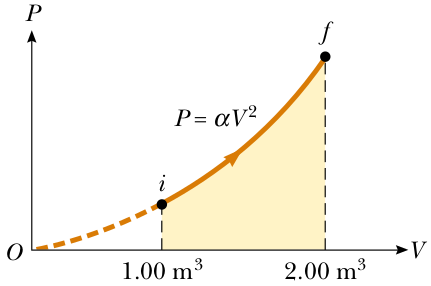
\includegraphics[scale=0.4]{17}
	%\end{figure}
	\begin{figure}[H]
		\centering
		\begin{tikzpicture}[scale=0.8]
		\begin{scope}
		\coordinate [label=above:$i$] (i) at (1,0.5);
		\coordinate [label=left:$f$] (f) at (3,4.4);
		\draw (0,0)-- (4,0);
		\draw [dashed] (0,0.5)-- (1,0.5);
		\draw [dashed] (1,0)--(1,0.5);
		\draw [dashed] (3,0)--(3,4.5);
		\draw [dashed] (0,0)--(1,.5);
		\draw (0,0)-- (0,4.5);
		\draw(0,4.2) node [color=blue, right=.1cm]{$P\left(Pa\right)$};
		\draw(4,0) node [color=blue, right=.1cm]{$V\left(m^{3}\right)$};
		\draw [arrows = {-Latex[width=8pt, length=10pt]}] (2,2) -- (2.2,2.4);
		\draw [arrows = {-Latex[width=8pt, length=8pt]}] (1.7,1.5) -- (1.2,3);
		\path[domain=1:3,name path=C]plot(\x,{0.5*\x*\x});
		\path[domain=1:3,name path=X](1,0)node[below]{$ 1.00 $}--(3,0)node[below]{$ 2.00 $};
		\tikzfillbetween[of={C and X}]{pattern=north east lines,pattern color=cyan!20!black};
		%\tikzfillbetween[of={C and X}]{pattern=bricks,pattern color=magenta};
		\draw[domain=1:3,samples=50,magenta]plot(\x,{0.5*\x*\x});
		\node[right,text=blue] at (0,3.3){$ \displaystyle P=\alpha V^{2}$};
		\draw (1,0.5) node {$\bullet$};
		\draw (3,4.5) node {$\bullet$};
		\end{scope}
		\end{tikzpicture}
	\end{figure}
	\item មួយម៉ូលនៃឧស្ម័ន $\ce{O2}$ សន្មតថាវាជាឧស្ម័នបរិសុទ្ធ។
	\begin{enumerate}[k]
		\item ឧស្ម័នរីកនៅសីតុណ្ហភាពថេរ $T=310K$ ពីមាឌដើម $V_i=12L$ ទៅ $V_f=19L$។\\
		គណនាកម្មន្តក្នុងដំណើរការរីកមាឌរបស់ឧស្ម័ន។
		\item ឧស្ម័នរួមមាឌនៅសីតុណ្ហភាពថេរ $T=310K$ ពីមាឌ $V_{i}=19L$ ទៅ $V_{f}=12L$។\\
		គណនាកម្មន្តក្នុងដំណើរការរួមមាឌរបស់ឧស្ម័ន។\\
		គេឲ្យៈ $\ln\left(\frac{19}{12}\right)=0.46,~\ln\left(\frac{12}{19}\right)=-0.46$ និង $R=8.31J/mol\cdot K$
	\end{enumerate}
	\begin{formula}
		\begin{enumerate}[m]
			\item \emph{\kml កម្មន្តក្នុងករណីមាឌថេរ(លំនាំអុីសូករ)}
			\begin{align*}
			\text{ករណី}\quad :&\quad V=\text{ថេរ}\quad \text{គេបាន}\quad W=0
			\end{align*}
			\item \emph{\kml ថាមពលក្នុង និងបម្រែបម្រួលថាមពលក្នុងនៃឧស្ម័នៈ}
			\begin{enumerate}[k,2]
				\item ថាមពលក្នុងនៃឧស្ម័នៈ\\ គឺជាថាមពលសុីនេទិចសរុបនៃឧស្ម័ន។
				\begin{align*}
					\text{គេបាន}\quad:&\quad U=\frac{3}{2}nRT\\
					\text{ឬ}\quad:&\quad U=\frac{3}{2}Nk_{B}T
				\end{align*}
				\item បម្រែបម្រួលថាមពលក្នុងនៃឧស្ម័ន
				\begin{align*}
					\text{យើងបាន}\quad:&\quad \Delta U=U_{2}-U_{1}\\
					\text{នោះ}\quad:&\quad \Delta U =\frac{3}{2}nRT_{2}-\frac{3}{2}nRT_{1}\\
					\text{ដូចនេះ}\quad:&\quad \Delta U = \frac{3}{2}nR\Delta T
				\end{align*}
			\end{enumerate}
			\item \emph{\kml ច្បាប់ទី១ ទែម៉ូឌីណាមិចៈ}
			កម្តៅស្រូបដោយប្រព័ន្ធស្មើនឹងផលបូកកម្មន្តបង្កើតឡើងដោយប្រព័ន្ធ និងបម្រែបម្រួលថាមពលក្នុងនៃប្រព័ន្ធ។
				\begin{align*}
					\text{គេកំណត់សរសេរ}\quad :&\quad Q=W+\Delta U
				\end{align*}
			\item \emph{\kml កម្មន្តក្នុងករណីកម្តៅមិនប្តូរជាមួយមជ្ឍដ្ឋានក្រៅ(លំនាំអាដ្យាបាទិច)} ជាលំនាំមួយដែលគ្មានបណ្តូរ​ថាមពលកម្តៅ (មិនស្រូប និងមិនបញ្ចេញកម្តៅ) ជាមួយមជ្ឍដ្ឋានក្រៅ មានន័យថា $Q=0J$។
			\begin{align*}
				\text{តាមច្បាប់ទីមួយទែម៉ូឌីណាមិច}\quad :&\quad Q=W+\Delta U\quad\text{តែ}\quad Q=0\\
				\text{ដូចនេះ}\quad :&\quad W=-\Delta U
			\end{align*}
		\end{enumerate}
	\end{formula}
	\item នៅលក្ខខណ្ឌ {\en (STP)} ឧស្ម័ន $2.2mol$ ត្រូវបានបង្រួមមាឌពី $50L$ ទៅ​ $10L$ តាមលំនាំអុីសូទែម។
	\begin{enumerate}[k]
		\item គណនាកម្មន្តដែលធ្វើលើឧស្ម័ន។ គេឲ្យៈ $\ln\left(0.2\right)=-1.61$។
		\item គណនាកម្តៅដែលភាយចេញពីឧស្ម័ន។
	\end{enumerate}
	\item ម៉ាសុីនកម្តៅមួយបានបំពេញកម្មន្ត $250J$ ក្នុងរយៈពេលដែលថាមពលក្នុងរបស់ម៉ាសុីនថយចុះ $500J$។\\ តើក្នុងលំនាំនេះកម្តៅនៃប្រព័ន្ធមានតម្លៃប៉ុន្មាន?
	\item ចូរគណនាបម្រែបម្រួលថាមពលក្នុងរបស់ប្រព័ន្ធឧស្ម័នទែម៉ូឌីណាមិចពេលៈ
	\begin{enumerate}[k]
		\item ប្រព័ន្ធស្រូបបរិមាណកម្តៅ $2000J$ និងធ្វើកម្មន្ត $500J$។
		\item ប្រព័ន្ធស្រូបបរិមាណកម្តៅ $1200J$ និងទទួលកម្មន្ត $400J$។
		\item បរិមាណកម្តៅ $300J$ ត្រូវបានបំភាយចេញពីប្រព័ន្ធនៅពេលមាឌថេរ។
	\end{enumerate}
	\item គណនាបម្រែបម្រួលថាមពលក្នុងនៃប្រព័ន្ធក្នុងករណីនីមួយៗខាងក្រោមៈ
	\begin{enumerate}[k]
		\item ប្រព័ន្ធស្រូបកម្តៅ $5kcal$ និងបំពេញកម្មន្ត $7200J$។
		\item ប្រព័ន្ធស្រូបកម្តៅ $5kcal$ និងរងនូវកម្មន្ត $7200J$។
		\item ប្រព័ន្ធឧស្ម័នមានមាឌថេរ និងបំភាយកម្តៅអស់ $4kcal$។
	\end{enumerate}
	\item គេធ្វើកម្មន្ត $25kJ$ លើប្រព័ន្ធឧស្ម័ន។ ក្រោយមកកម្តៅ $1.5kcal$ បានភាយចេញពីប្រព័ន្ធ។ \\គណនាបម្រែបម្រួលថាមពលក្នុង។ $\left(1cal=4.186J\right)$ 
	\item ក្នុងប្រព័ន្ធទែម៉ូឌីណាមិចប្រព័ន្ធទទួលកម្មន្ត $200J$​និងទទួលកម្តៅ $500J$។ រកបម្រែបម្រួលថាមពលក្នុង។
	\item ចូរគណនាបម្រែបម្រួលថាមពលក្នុងរបស់ប្រព័ន្ធៈ
	\begin{enumerate}[k]
		\item ប្រព័ន្ធស្រូបបរិមាណកម្តៅ $500cal$ និងធ្វើកម្មន្ត $400J$។
		\item ប្រព័ន្ធស្រូបកម្តៅ $300cal$ និងទទួលកម្មន្ត $420J$។
		\item បរិមាណកម្តៅ $1200cal$ ត្រូវបានភាយចេញពីប្រព័ន្ធនៅពេលមាឌថេរ។ គេឲ្យ $1cal=4.19J$
	\end{enumerate}
	\item ចូរគណនាបម្រែបម្រួលថាមពលក្នុងរបស់ប្រព័ន្ធៈ
	\begin{enumerate}[k]
		\item ប្រព័ន្ធធ្វើកម្មន្ត $5.0J$ ខណៈវារីកអាដ្យាបាទិច។
		\item ខណៈប្រព័ន្ធរួមអាដ្យាបាទិច កម្មន្ត $80J$ ត្រូវបានធ្វើលើឧស្ម័ន។
	\end{enumerate}
	\item ឧស្ម័នមួយស្រូបយកកម្តៅ $6.4kJ$ និងបំពេញកម្មន្ត $1200J$ ក្នុងពេលលំនាំនេះវាបានបញ្ចេញកម្តៅទៅវិញ $2400J$។ គណនាបម្រែបម្រួលថាមពលក្នុងរបស់ឧស្ម័ន។
	\item ឧស្ម័នមួយមានមាឌ $10L$ ស្ថិតនៅក្រោមសម្ពាធ $2\times10^{5}Pa$ និងសីតុណ្ហភាព $20^\circ C$។ ក្នុងលំនាំអុីសូបារ ឧស្ម័ននោះបានស្រូបបរិមាណកម្តៅ $5000J$ ហើយថាមពលក្នុងរបស់វាកើន $2000J$។ គណនាៈ
	\begin{enumerate}[k,2]
		\item កម្មន្តដែលបានបំពេញដោយឧស្ម័ននោះ។
		\item មាឌនៃឧស្ម័ននៅភាពស្រេច។
		\item សីតុណ្ហភាពស្រេចនៃឧស្ម័ននោះ។
	\end{enumerate} 
	\item ក្នុងសុីឡាំងមួយមានឧស្ម័នបរិសុទ្ធម៉ូណូអាតូម $0.5mol$។ គេធ្វើឲ្យឧស្ម័ននេះរីកមាឌពី $5dm^3$ ទៅ​ $12.5dm^3$ តាមលំនាំអុីសូទែម។ គេដឹងថាកម្មន្តដែលបានធ្វើដោយឧស្ម័ន ក្នុងរយៈពេលនៃដំណើរការគឺ $1142J$។\\គេឲ្យៈ $R=8.31J/mol\cdot K$
	\begin{enumerate}[k]
		\item គណនាសីតុណ្ហភាពនៃឧស្ម័នក្នុងពេលដំណើរការ។
		\item គណនាថាមពលក្នុងនៃឧស្ម័ននៅត្រង់ទីតាំងស្រេច។
		\item គណនាថាមពលកម្តៅដែលស្រូបដោយប្រព័ន្ធក្នុងរយៈពេលនៃដំណើរការ។
	\end{enumerate}
	\item ចូរគណនាកម្មន្តតាមលំនាំនីមួយៗ​ និងកម្មន្តសរុបក្នុងដ្យាក្រាម $P-V$ ខាងក្រោមៈ
	\begin{figure}[H]
		\centering
		\begin{tikzpicture}[scale=1]
		\begin{scope}
		\draw [dashed,gray,very thin, xstep=1.0cm,ystep=1.0cm] grid (3.5,3.5);
		\fill [cyan!60] (2,0) -- (2,3) -- (3,3) -- (3,0) -- cycle;
		\pattern[pattern color=white,pattern=bricks] (2,0) -- (2,3) -- (3,3) -- (3,0) -- cycle;
		\fill [cyan!60] (1,0) -- (2,2) -- (2,0) -- cycle;
		\pattern[pattern color=white,pattern=bricks] (1,0) -- (2,2) -- (2,0) -- cycle;
		\draw (0,0)-- (4,0);
		\draw [dashed] (0,2)-- (2,2);
		\draw [dashed] (0,3)-- (3,3);
		\draw [ultra thick] (2,3)-- (3,3);
		\draw [ultra thick] (1,0)-- (2,2);
		\draw [ultra thick] (2,2)-- (2,3);
		\draw [dashed] (3,2)-- (3,3);
		\draw [dashed] (2,0)--(2,2);
		\draw [dashed] (3,2)-- (3,0);
		\draw (0,0)-- (0,4);
		\draw(0,3.9) node [color=blue, right=.1cm]{$P\left(kPa\right)$};
		\draw(0,2) node [color=blue, left=.1cm]{$140$};
		\draw(0,3) node [color=blue, left=.1cm]{$210$};
		\draw (1,-.3) node [color=blue]{$0.25$};
		\draw (2,-.3) node [color=blue]{$0.50$};
		\draw (3,-.3) node [color=blue]{$0.80$};
		\draw (4,0) node [color=blue, right=.1cm]{$V\left(m^{3}\right)$};
		\draw [arrows = {-Latex[width=10pt, length=10pt]}] (2.2,3) -- (2.7,3);
		\draw [arrows = {-Latex[width=10pt, length=10pt]}] (2,2.5) -- (2,2.7);
		\draw [arrows = {-Latex[width=10pt, length=10pt]}] (1.5,1) -- (1.7,1.4);
		\draw (1,0) node {$\bullet$};
		\draw (3,3) node {$\bullet$};
		\coordinate [label=above left:$A$] (A) at (1,0);
		\coordinate [label=above right:$B$] (B) at (3,3);
		\coordinate [label=left:$1$] (1) at (1.4,1.1);
		\coordinate [label=left:$2$] (2) at (1.9,2.5);
		\coordinate [label=above:$3$] (3) at (2.5,3);
		\end{scope}
		\end{tikzpicture}
	\end{figure}
	\item \begin{enumerate}[k]
		\item គណនាកម្មន្តដែលបានធ្វើដោយឧស្ម័នបរិសុទ្ធម៉ូណូអាតូម ដែលចេញពីចំណុច $A$ ទៅចំណុច $B$\\ដូចដែលបានបង្ហាញក្នុងរូប។
		\item បើសិនជានៅត្រង់ចំណុច $A$ សីតុណ្ហភាពនៃឧស្ម័នមានតម្លៃ $267K$។ \\តើវាមានសីតុណ្ហភាពប៉ុន្មានពេលនៅត្រង់ចំណុច $C$។
		\item តើបរិមាណកម្តៅប៉ុន្មានដែលត្រូវបានស្រូប ឬបញ្ចេញពីឧស្ម័នក្នុងកំឡុងពេលដំណើរការនេះ?
	\end{enumerate}
	\begin{figure}[H]
		\centering
		\begin{tikzpicture}[scale=1]
		\begin{scope}
		\draw [dashed,gray,very thin, xstep=1.0cm,ystep=1.0cm] grid (5.5,3.5);
		\fill [cyan!60] (1,0) -- (1,1) -- (2,1) -- (3,3) --(3,3) -- (4,2) -- (4,1)--(5,1) -- (5,0) -- cycle;
		\pattern[pattern color=white,pattern=bricks] (1,0) -- (1,1) -- (2,1) -- (3,3) --(3,3) -- (4,2) -- (4,1)--(5,1) -- (5,0) -- cycle;
		\draw (0,0)-- (6,0);
		\draw [ultra thick] (1,1)-- (2,1)--(3,3)--(4,2)--(4,1)--(5,1);
		\draw [dashed] (1,0)--(1,1);
		\draw [dashed] (5,1)-- (5,0);
		\draw (0,0)-- (0,4);
		\draw(0,3.9) node [color=blue, right=.1cm]{$P\left(kPa\right)$};
		\draw(0,1) node [color=blue, left=.1cm]{$200$};
		\draw(0,2) node [color=blue, left=.1cm]{$400$};
		\draw(0,3) node [color=blue, left=.1cm]{$600$};
		\draw (1,-.3) node [color=blue]{$2.0$};
		\draw (2,-.3) node [color=blue]{$4.0$};
		\draw (3,-.3) node [color=blue]{$6.0$};
		\draw (4,-.3) node [color=blue]{$8.0$};
		\draw (5,-.3) node [color=blue]{$10$};
		\draw (6,0) node [color=blue, right=.1cm]{$V\left(m^{3}\right)$};
		\draw [arrows = {-Latex[width=10pt, length=10pt]}] (3.4,2.6) -- (3.6,2.4);
		\draw [arrows = {-Latex[width=10pt, length=10pt]}] (2.5,2) -- (2.6,2.2);
		\draw [arrows = {-Latex[width=10pt, length=10pt]}] (4.5,1) -- (4.7,1);
		\draw [arrows = {-Latex[width=10pt, length=10pt]}] (1.5,1) -- (1.7,1);
		\draw (1,1) node {$\bullet$};
		\draw (3,3) node {$\bullet$};
		\draw (5,1) node {$\bullet$};
		\coordinate [label=above left:$A$] (A) at (1,1);
		\coordinate [label=above right:$B$] (B) at (3,3);
		\coordinate [label=above right:$C$] (C) at (5,1);
		\end{scope}
		\end{tikzpicture}
	\end{figure}
	\item គណនាកម្មន្តសរុបក្នុងបម្លែងបិទ $ABCA$?
	\begin{figure}[H]
		\centering
		\begin{tikzpicture}
			\begin{scope}
				\draw (0,0)-- (0,4);
				\draw (0,0)-- (4,0);
				\draw [ultra thick] (1,1) -- (1,3) -- (3,1) --cycle;
				\coordinate [label=above:$A$] (A) at (1,3);
				\coordinate [label=right:$B$] (B) at (3,1);
				\coordinate [label=above left:$C$] (C) at (1,1);
				\draw [dashed] (1,0) --(1,1);
				\draw [dashed] (0,1) --(1,1);
				\draw [dashed] (0,3) --(1,3);
				\draw [dashed] (3,0) --(3,1);
				\fill [cyan!60] (1,1) -- (1,3) -- (3,1)--cycle;
				\pattern [pattern color=white, pattern=bricks] (1,1) -- (1,3) -- (3,1)--cycle;
				\coordinate [label=right:$V$] ($V$) at (4,0);
				\coordinate [label=below:$2.0m^{3}$] ($V_{1}$) at (1,0);
				\coordinate [label=below:$5.0m^{3}$] ($V_{2}$) at (3,0);
				\coordinate [label=left:$P$] ($P$) at (0,4);
				\coordinate [label=left:$1.0 atm$] ($P_{1}$) at (0,1);
				\coordinate [label=left:$2.0 atm$] ($P_{2}$) at (0,3);
				\draw [arrows = {-Latex[width=10pt, length=10pt]}] (1,2) -- (1,2.2);
				\draw [arrows = {-Latex[width=10pt, length=10pt]}] (2,1) -- (1.8, 1);
				\draw [arrows = {-Latex[width=10pt,length=10pt]}] (2,2)--(2.2,1.8);
			\end{scope}
		\end{tikzpicture}
	\end{figure}
	\item ឧស្ម័នបរិសុទ្ធមួយធ្វើបម្លែងបិទពីភាព $A$ រួចទៅភាព $B$ រួចទៅភាព $C$ ហើយទៅភាព $D$ ទៀត។ ក្រោយត្រឡប់មកភាពដើមវិញដូចបង្ហាញក្នុងរូប។ ចូរគណនាៈ
	\begin{multicols}{2}
		\begin{enumerate}[k]
			\item គណនាកម្មន្ត $AB,~BC,~CD$ និង $DA$។
			\item កម្មន្តសរុបក្នុងបម្លែងបិទ។
			\item កម្តៅដែលទទួលបានក្នុងបម្លែងបិទ។
		\end{enumerate}
		\begin{figure}[H]
			\centering
			\begin{tikzpicture}[scale=1]
			\begin{scope}
			\draw (0,0)-- (0,4);
			\draw (0,0)-- (4,0);
			\draw [ultra thick] (1,1) -- (1,3) -- (3,3) --(3,1) --cycle;
			\coordinate [label=above:$A$] (A) at (1,3);
			\coordinate [label=above:$B$] (B) at (3,3);
			\coordinate [label=right:$C$] (C) at (3,1);
			\coordinate [label=below left:$D$] (D) at (1,1);
			\draw [dashed] (1,0) --(1,1);
			\draw [dashed] (0,1) --(1,1);
			\draw [dashed] (0,3) --(1,3);
			\draw [dashed] (3,0) --(3,1);
			\fill [cyan!60] (1,1) -- (1,3) -- (3,3) -- (3,1)--cycle;
			\pattern [pattern color=white, pattern=bricks] (1,1) -- (1,3) -- (3,3) -- (3,1)--cycle;
			\coordinate [label=right:$V\left(L\right)$] ($V$) at (4,0);
			\coordinate [label=below:$2.0$] ($V_{1}$) at (1,0);
			\coordinate [label=below:$4.0$] ($V_{2}$) at (3,0);
			\coordinate [label=left:$P\left(atm\right)$] ($P$) at (0,4);
			\coordinate [label=left:$1.0$] ($P_{1}$) at (0,1);
			\coordinate [label=left:$2.0$] ($P_{2}$) at (0,3);
			\draw [arrows = {-Latex[width=10pt, length=10pt]}] (1,2) -- (1,2.2);
			\draw [arrows = {-Latex[width=10pt, length=10pt]}] (2,1) -- (1.8, 1);
			\draw [arrows = {-Latex[width=10pt,length=10pt]}] (3,2)--(3,1.8);
			\draw [arrows = {-Latex[width=10pt,length=10pt]}] (2.3,3)--(2.5,3);
			\end{scope}
			\end{tikzpicture}
		\end{figure}
	\end{multicols}
	\item ឧស្ម័នមួយស្ថិតក្នុងសុីឡាំងបិទជិតដោយពីស្តុងដែលអាចផ្លាស់ទីដោយគ្មានកកិត និងស្ថិតក្រោមសម្ពាធបរិយាកាស។ នៅពេលដែលកម្តៅ $254kcal$​ត្រូបានផ្តល់ឲ្យឧស្ម័ន មាឌរបស់វាកើនឡើងពី $12.0m^{3}$ ទៅដល់​ $16.2m^{3}$។
	\begin{enumerate}[k]
		\item គណនាកម្មន្តដែលបំពេញដោយឧស្ម័ន។
		\item គណនាបម្រែបម្រួលថាមពលក្នុងនៃឧស្ម័ន។
	\end{enumerate}
	\item គេបញ្ចុះសីតុណ្ហភាពអេល្យូមដែលមានមាឌដើម $1.0m^{3}$ នៅសីតុណ្ហភាព $0^\circ C$ និងសម្ពាធថេរ $1.0atm$ រហូតដល់ត្រឹមមាឌ $0.75m^{3}$។ គណនាបរិមាណកម្តៅ។
	\item ដូចបង្ហាញក្នុងរូប ឧស្ម័នរីកមាឌពី $V_{0}$ ទៅ $4V_{0}$ ហើយសម្ពាធថយចុុះពី $P_{0}$ ទៅ $P_{0}=\frac{P_{0}}{4}$។ គេដឹងថា $V_{0}=1.0m^{3}$  ហើយ $P_{0}=40Pa$។ ចូរគណនាកម្មន្តដែលបំពេញដោយឧស្ម័នប្រសិនបើសម្ពាធ និងមាឌឧស្ម័នប្រែប្រួល។
	\begin{multicols}{2}
		\begin{enumerate}[k]
			\item តាមគន្លង $\left(A\right)$។
			\item តាមគន្លង $\left(B\right)$។
			\item តាមគន្លង $\left(C\right)$។
		\end{enumerate}
		\begin{figure}[H]
			\centering
			\begin{tikzpicture}[scale=1]
			\begin{scope}
			\draw [dashed,gray,very thin, xstep=1.0cm,ystep=1.0cm] grid (4.5,4.5);
			\draw (0,0)-- (0,4.5);
			\draw (0,0)-- (4.5,0);
			\draw [color=magenta, ultra thick] (4,1) -- (1,1) -- (1,4);
			\draw [color=green!30!black, ultra thick] (1,4) -- (4,4) -- (4,1);
			\draw [color=yellow!10!orange, ultra thick] (1,4) -- (4,1);
			\coordinate [label=below:$0$] (0) at (0,0);
			\coordinate [label=above:$A$] (A) at (2.5,4);
			\coordinate [label=above right:$B$] (B) at (2,3);
			\coordinate [label=right:$C$] (C) at (1,2.5);
			\coordinate [label=below:$V_{0}$] ($V_{0}$) at (1,0);
			\coordinate [label=below:$4V_{0}$] ($V_{4}$) at (4,0);
			\coordinate [label=left:$P_{0}$] ($P_{0}$) at (0,4);
			\draw [color=magenta, arrows = {-Latex[width=10pt, length=10pt]}] (1,2.5) -- (1,2.3);
			\draw [color=magenta, arrows = {-Latex[width=10pt, length=10pt]}] (2.5,1) -- (2.7, 1);
			\draw [color=yellow!10!orange, arrows = {-Latex[width=10pt,length=10pt]}] (2.5,2.5)--(2.6,2.4);
			\draw [color=green!30!black, arrows = {-Latex[width=10pt,length=10pt]}] (2.5,4)--(2.7,4);
			\draw [color=green!30!black, arrows = {-Latex[width=10pt, length=10pt]}] (4,2.5) -- (4,2.3);
			\draw [color=black] (1,4) node {$\bullet$};
			\draw [color=black] (4,1) node {$\bullet$};
			\end{scope}
			\end{tikzpicture}
		\end{figure}
	\end{multicols}
	\item \begin{multicols}{2}
		ឧស្ម័នមួយនៅក្នុងធុងបិទជិត ដំណើរការក្នុងវដ្តដូចបង្ហាញក្នុងលើក្រាប $P-V$។ មាត្រដ្ឋានដេកកំណត់ឲ្យតម្លៃ $V_{s}=4.0m^{3}$ និងមាត្រដ្ឋានឈរកំណត់ឲ្យសម្ពាធគិតជា $\left(N/m^{2}\right)$។\\ គណនាថាមពលកម្តៅក្នុងមួយដំណើរការពេញនៃវដ្ត។
			\begin{figure}[H]
			\centering
			\begin{tikzpicture}[scale=1]
			\begin{scope}
			\draw [dashed,gray,very thin, xstep=1.0cm,ystep=1.0cm] grid (4.5,4.5);
			\draw (0,0)-- (0,4.5);
			\draw (0,0)-- (4.5,0);
			\draw [color=magenta, ultra thick] (1,1) -- (4,3) -- (1,3)--cycle;
			\coordinate [label=below:$A$] (A) at (1,1);
			\coordinate [label=above:$B$] (B) at (4,3);
			\coordinate [label=above:$C$] (C) at (1,3);
			\coordinate [label=below:$0$] (0) at (0,0);
			\coordinate [label=below:$V_{s}$] ($V_{s}$) at (4,0);
			\coordinate [label=left:$40$] ($40$) at (0,4);
			\coordinate [label=left:$30$] ($30$) at (0,3);
			\coordinate [label=left:$20$] ($20$) at (0,2);
			\coordinate [label=left:$10$] ($10$) at (0,1);
			\draw [color=magenta, arrows = {-Latex[width=10pt, length=10pt]}] (2.5,2) -- (2.7,2.1);
			\draw [color=magenta, arrows = {-Latex[width=10pt,length=10pt]}] (2.5,3)--(2.3,3);
			\draw [color=magenta, arrows = {-Latex[width=10pt, length=10pt]}] (1,2) -- (1,1.8);
			\draw [color=black] (1,1) node {$\bullet$};
			\draw [color=black] (4,3) node {$\bullet$};
			\draw [color=black] (1,3) node {$\bullet$};
			\end{scope}
			\end{tikzpicture}
		\end{figure}
	\end{multicols}
	\item គេធ្វើកម្មន្តលើប្រព័ន្ធមួយ $200J$ ហើយកម្តៅ $70.0cal$ ត្រូវបានភាយចេញពីប្រព័ន្ធ។ \\ដោយប្រើច្បាប់ទីមួយទែម៉ូឌីណាមិចៈ
	\begin{enumerate}[k]
		\item ទាញរកកម្មន្ត $\left(W\right)$ ដោយបញ្ជាក់សញ្ញា និងពន្យល់ហេតុផល។
		\item កំណត់សញ្ញា $\left(Q\right)$ ព្រមទាំងពន្យល់ហេតុផល។
		\item គណនាបម្រែបម្រួលថាមពលក្នុង $\left(\Delta U\right)$។ តើថាមពលក្នុងថយចុះ ឬកើនឡើង?
	\end{enumerate}
	\item \begin{enumerate}[k]
		\item ពិសីរត់ហាត់ប្រាណតាមបណ្តោយឆ្នេរសមុទ្រដោយបំពេញកម្មន្ត $4.3\times10^{5}J$ និងបញ្ចេញកម្តៅ $3.8\times10^{5}J$។ គណនាបម្រែបម្រួលថាមពលក្នុង ក្នុងខ្លួនពិសី។
		\item បើនាងប្តូរពីរត់មកដើរវិញ នោះនាងបញ្ចេញកម្តៅអស់ $1.2\times10^{5}J$ និងថាមពលក្នុងថយចុះអស់ $2.6\times10^{5}J$។ តើកំឡុងពេលដើរ ពិសីបំពេញកម្មន្តបានប៉ុន្មាន?
	\end{enumerate}
	\item ក្នុងសុីឡាំងមួយមានឧស្ម័នបរិសុទ្ធម៉ូណូអាតូម $0.5mol$ នៅសីតុណ្ហភាព $310K$។\\ ដោយរក្សាសីតុណ្ហភាពថេរ ឧស្ម័នរីកមាឌពី $310dm^{3}$ រហូតដល់ $450dm^{3}$។ គេឲ្យៈ $\ln\left(1.45\right)=0.37$
	\begin{enumerate}[k,2]
		\item គណនាកម្មន្តដែលប្រព័ន្ធបញ្ចេញ។
		\item គណនាបម្រែបម្រួលថាមពលក្នុងរបស់ឧស្ម័ន។
		\item គណនាកម្តៅស្រូបដោយឧស្ម័នក្នុងពេលបម្រែបម្រួលមាឌ។
	\end{enumerate}
	\item គណនាបម្រែបម្រួលថាមពលក្នុងនៃប្រព័ន្ធក្នុងករណីនីមួយៗ ដូចខាងក្រោមៈ
	\begin{enumerate}[k]
		\item ប្រព័ន្ធស្រូបកម្តៅ $500cal$ និងបញ្ចេញកម្មន្ត $400J$។
		\item ប្រព័ន្ធស្រូមកម្តៅ $300cal$ និងរងកម្មន្ត $420J$។
		\item ប្រព័ន្ធឧស្ម័នមានមាឌថេរ និងបំភាយកម្តៅអស់ $1200cal$។
	\end{enumerate}
	\item ឧស្ម័នក្នុងធុងមួយមានសម្ពាធ $1.50atm$ និងមានមាឌ $4.00m^{3}$។ គណនាកម្មន្តៈ
	\begin{enumerate}[k]
		\item បើឧស្ម័នរីកមាឌពីរដងនៃមាឌដើម និងរក្សាសម្ពាធថេរ។
		\item បើគេបណ្ណែនឧស្ម័នមក $\frac{1}{4}$ នៃមាឌដើម និងសម្ពាធថេរ។
	\end{enumerate}
	\item ឧស្ម័នបរិសុទ្ធមួយត្រូវបានបង្រួមដោយសម្ពាធថេរ $0.8atm$ ពីមាឌ $9.0L$ ទៅ $2.0L$។\\
	ក្នុងលំនាំនេះឧស្ម័នបញ្ចេញកម្តៅ $400J$។ គណនាៈ
	\begin{enumerate}[k]
		\item កម្មន្តនៃដំណើរការរបស់ឧស្ម័ន។
		\item បម្រែបម្រួលថាមពលក្នុងរបស់ឧស្ម័ន។
	\end{enumerate} 
	\item ឧស្ម័នបរិសុទ្ធមួយមានសីតុណ្ហភាពដើម $300K$ រងបម្លែងទែម៉ូឌីណាមិចតាមលំនាំអុីសូបារពីមាឌ $1.00m^{3}$ ទៅ $3.00m^{3}$ នៅសម្ពាធ $2.50kPa$។ កម្តៅ $12.5kJ$ ត្រូវបានស្រូបដោយឧស្ម័ន។
	\begin{enumerate}[k]
		\item គណនាបម្រែប្រួលថាមពលក្នុងរបស់ឧស្ម័ន។
		\item សីតុណ្ហភាពចុងក្រោយរបស់ឧស្ម័ន។
	\end{enumerate} 
	\item ឧស្ម័នបរិសុទ្ធមួយត្រូវបានឆ្លងកាត់នៃវដ្តដំណើរការដូចរូប។
	\begin{multicols}{2}
		\begin{enumerate}[k]
			\item គណនាថាមពលកម្តៅសរុបក្នុងបម្លែងបិទ។
			\item បើឧស្ម័នប្រព្រឹត្តក្នុងវដ្តបញ្ច្រាស $ACBA$ វិញ។\\​
			គណនាថាមពលកម្តៅសរុបក្នុងវដ្តបញ្ច្រាស។
		\end{enumerate}
		\begin{figure}[H]
			\centering
			\begin{tikzpicture}[scale=1]
			\begin{scope}
			\draw [dashed,gray,very thin, xstep=1.0cm,ystep=1.0cm] grid (3.1,4.1);
			\draw (0,0)-- (0,4.5);
			\draw (0,0)-- (3.5,0);
			\fill [cyan!60] (1,1) -- (3,4) -- (3,1) --cycle;
			\pattern [pattern color=white, pattern=bricks] (1,1) -- (3,4) -- (3,1) --cycle;
			\draw [ultra thick] (1,1) -- (3,4) -- (3,1)--cycle;
			\coordinate [label=above left:$A$] (A) at (1,1);
			\coordinate [label=above:$B$] (B) at (3,4);
			\coordinate [label=right:$C$] (C) at (3,1);
			\coordinate [label=below:$0$] (0) at (0,0);
			\coordinate [label=right:$V\left(m^{3}\right)$] ($V$) at (3.5,0);
			\coordinate [label=below:$6.0$] ($6.0$) at (1,0);
			\coordinate [label=below:$8.0$] ($8.0$) at (2,0);
			\coordinate [label=below:$10$] ($10$) at (3,0);
			\coordinate [label=above:$P\left(kPa\right)$] ($P$) at (0,4.5);
			\coordinate [label=left:$8.0$] ($8.0$) at (0,4);
			\coordinate [label=left:$6.0$] ($6.0$) at (0,3);
			\coordinate [label=left:$4.0$] ($4.0$) at (0,2);
			\coordinate [label=left:$2.0$] ($2.0$) at (0,1);
			\draw [arrows = {-Latex[width=10pt, length=10pt]}] (3,2.5) -- (3,2.3);
			\draw [arrows = {-Latex[width=10pt,length=10pt]}] (2,1)--(1.8,1);
			\draw [arrows = {-Latex[width=10pt, length=10pt]}] (2,2.5) -- (2.1,2.6);
			\draw [color=black] (1,1) node {$\bullet$};
			\draw [color=black] (3,1) node {$\bullet$};
			\draw [color=black] (3,4) node {$\bullet$};
			\draw [dashed] (0,1)--(1,1);
			\draw [dashed] (0,4)--(3,4);
			\draw [dashed] (1,0)--(1,1);
			\draw [dashed] (3,0)--(3,1);
			\end{scope}
			\end{tikzpicture}
		\end{figure}
	\end{multicols}
	\item ក្នុងរូបបង្ហាញពីវដ្តនៃឧស្ម័ន។ បម្រែបម្រួលថាមពលក្នុងនៃឧស្ម័នក្នុងលំនាំពី $a\rightarrow c$ តាមគន្លង $abc$ គឺ $-200J$។ ថាមពល $180J$ ត្រូវបានផ្តល់ជាកម្តៅក្នុងលំនាំពី $c\rightarrow d$។\\ ម្យ៉ាងទៀតថាមពល $80J$ ត្រូវបានផ្តល់ជាកម្តៅក្នុងលំនាំពី $d\rightarrow a$។\\ ចូរគណនាកម្មន្តដែលបំពេញដោយឧស្ម័នក្នុងលំនាំពី $c\rightarrow d$។
		\begin{figure}[H]
		\centering
		\begin{tikzpicture}[scale=1.5]
		\begin{scope}
		\draw (0,0)-- (0,3.5);
		\draw (0,0)-- (3.5,0);
		\draw [ultra thick] (1,1) -- (3,1) -- (3,3) -- (1,2) --cycle;
		\coordinate [label=above:$a$] (a) at (3,3);
		\coordinate [label=above left:$b$] (b) at (1,2);
		\coordinate [label=left:$c$] (c) at (1,1);
		\coordinate [label=right:$d$] (c) at (3,1);
		\coordinate [label=right:$V$] ($V$) at (3.5,0);
		\coordinate [label=above:$P$] ($P$) at (0,3.5);
		\draw [arrows = {-Latex[width=10pt, length=10pt]}] (3,2) -- (3,2.2);
		\draw [arrows = {-Latex[width=10pt,length=10pt]}] (2,1)--(2.2,1);
		\draw [arrows = {-Latex[width=10pt,length=10pt]}] (1,1.5)--(1,1.3);
		\draw [arrows = {-Latex[width=10pt, length=10pt]}] (2,2.5) -- (1.6,2.3);
		\end{scope}
		\end{tikzpicture}
	\end{figure}
	\newpage
	\item ឧស្ម័នមួយត្រូវបានដាក់ឲ្យដំណើរការក្នុងវដ្ត $abca$ ដូចបង្ហាញក្នុងដ្យាក្រាម $\left(P-V\right)$។ កម្មន្តសរុបក្នុងបម្លែងបិទគឺ $1.2J$។ ក្នុងលំនាំ $ab$ បម្រែបម្រួលថាមពលក្នុងមានតម្លៃ $3.0J$​និងកម្មន្តបំពេញដោយឧស្ម័នគឺ $5.0J$។\\ ក្នុងលំនាំ $ca$ ថាមពល $2.5J$ ត្រូវបានផ្តល់ជាកម្តៅ។ ចូរគណនាថាមពលកម្តៅៈ
	\begin{multicols}{2}
		\begin{enumerate}
			\item ក្នុងលំនាំ $ab$។ 
			\item ក្នុងលំនាំ $bc$។
		\end{enumerate}
		\begin{figure}[H]
			\centering
			\begin{tikzpicture}[scale=1]
			\begin{scope}
			\draw (0,0)-- (0,3.5);
			\draw (0,0)-- (3.5,0);
			\draw [ultra thick] (1,1) -- (1,3) -- (3,3) -- cycle;
			\coordinate [label=above:$a$] (a) at (1,3);
			\coordinate [label=above:$b$] (b) at (3,3);
			\coordinate [label=below:$c$] (c) at (1,1);
			\coordinate [label=right:$V$] ($V$) at (3.5,0);
			\coordinate [label=above:$P$] ($P$) at (0,3.5);
			\draw [arrows = {-Latex[width=10pt,length=10pt]}] (2,3)--(2.2,3);
			\draw [arrows = {-Latex[width=10pt,length=10pt]}] (1,2)--(1,2.2);
			\draw [arrows = {-Latex[width=10pt, length=10pt]}] (2,2) -- (1.8,1.8);
			\end{scope}
			\end{tikzpicture}
		\end{figure}
	\end{multicols}
	\item កន្លះម៉ូលនែឧស្ម័នបរិសុទ្ធមួយត្រូវបានដំណើរការពីភាព $a$ ទៅភាព $c$ ដូចបង្ហាញក្នុងរូប។
	\begin{multicols}{2}
		\begin{enumerate}[k]
			\item គណនាសីតុណ្ហភាពស្រេចនៃឧស្ម័ន។
			\item គណនាកម្មន្តដែលបានធ្វើលើ ឬធ្វើដោយ ឧស្ម័នដែលចេញពីភាព $a$ ទៅ $c$។
			\item តើកម្តៅត្រូវបានភាយចេញពីប្រព័ន្ធ ឬស្រូបចូលប្រព័ន្ធក្នុងដំណើរការនេះ?\\
			តើបរិមាណកម្តៅមានតម្លៃប៉ុន្មាន? ចូរពន្យល់។
		\end{enumerate}
		\begin{figure}[H]
			\centering
			\begin{tikzpicture}[scale=1.2]
			\begin{scope}
			\draw [dashed,magenta, ultra thick, xstep=1.0cm] grid (4.1,.1);
			\draw [dashed,magenta,ultra thick, ystep=1.5cm] grid (.1,3.1);
			\draw [ultra thick, ystep=1.5cm] (0,0)-- (0,3.5);
			\draw [ultra thick, xstep=1.0cm] (0,0)-- (4.5,0);
			\draw [ultra thick] (2,3) -- (3,1.5);
			\draw [ultra thick, color=cyan] (3,1.5) -- (4,1.5);
			\coordinate [label=above:$a$] (a) at (2,3);
			\coordinate [label=below:$b$] (b) at (3,1.5);
			\coordinate [label=below:$c$] (c) at (4,1.5);
			\coordinate [label=right:$V\left(m^{3}\right)$] ($V$) at (4.5,0);
			\coordinate [label=above:$P\left(Pa\right)$] ($P$) at (0,3.5);
			\coordinate [label=left:$4.0\times10^5$] ($P$) at (0,3);
			\coordinate [label=left:$2.0\times10^5$] ($P$) at (0,1.5);
			\draw [arrows = {-Latex[width=10pt,length=10pt]}] (2.42,2.4)--(2.5,2.3);
			\draw [color=cyan, arrows = {-Latex[width=10pt, length=10pt]}] (3.5,1.5) -- (3.7,1.5);
			\coordinate [label=below:$0.001$] ($0.001$) at (1,0);
			\coordinate [label=below:$0.002$] ($0.002$) at (2,0);
			\coordinate [label=below:$0.003$] ($0.003$) at (3,0);
			\coordinate [label=below:$0.004$] ($0.004$) at (4,0);
			\draw [color=blue] (2,3) node {$\bullet$};
			\draw [color=blue] (3,1.5) node {$\bullet$};
			\draw [color=blue] (4,1.5) node {$\bullet$};
			\end{scope}
			\end{tikzpicture}
		\end{figure}
	\end{multicols}
	\item ពីរម៉ូលនៃឧស្ម័នបរិសុទ្ធមួយត្រូវបានកំដៅក្រោមសម្ពាធថេរ ពី $27^\circ C$ ទៅ $107^\circ C$។
	\begin{enumerate}[k]
		\item គូសដ្យាក្រាម $P-V$ សម្រាប់ដំណើរការនេះ។
		\item គណនាកម្មន្តដែលបានធ្វើដោយឧស្ម័ន។
	\end{enumerate}
	\item ប្រាំមួយម៉ូលនៃឧស្ម័នបរិសុទ្ធមួយស្ថិតនៅក្នុងស៊ីឡាំងបិទជិតដោយពីស្តុងដែលអាចចល័តបាន។ នៅភាពដើមសីតុណ្ហភាពរបស់ឧស្ម័នគឺ $27.0^\circ C$ និងស្ថិតក្រោមសម្ពាធថេរ។\\ គណនាសីតុណ្ហភាពស្រេចនៃឧស្ម័នបន្ទាប់ពីវាបានធ្វើកម្មន្ត $1.75\times10^{3}J$។ 
	\item ពីរម៉ូលនៃឧស្ម័នបរិសុទ្ធមួយត្រូវបានបង្រួមមាឌដោយដាក់ក្នុងសុីឡាំងមួយ ដោយរក្សាសីតុណ្ហភាពថេរ $85^\circ C$ រហូតដល់សម្ពាធដើមរបស់វាកើនឡើងបីដង។
	\begin{enumerate}[k]
		\item គូសដ្យាក្រាម $P-V$ សម្រាប់ដំណើរការនេះ។
		\item គណនាកម្មន្តដែលបានបំពេញដោយឧស្ម័ន។
	\end{enumerate}
	\item ចូរសរសេរទំនាក់ទំនង់កម្មន្តបំពេញដោយឧស្ម័នចេញពីភាព $\left(A\right)\rightarrow \left(C\right)$ (ក្នុងរូប) ក្នុងករណីៈ
	\begin{multicols}{2}
		\begin{enumerate}[k]
			\item ឧស្ម័នដំណើរការតាមគន្លង $ADC$។
			\item ឧស្ម័នដំណើរការតាមគន្លង $ABC$។
			\item ឧស្ម័នដំណើរការតាមគន្លងត្រង់ $AC$។
		\end{enumerate}
		\begin{figure}[H]
			\centering
			\begin{tikzpicture}[scale=0.9]
			\begin{scope}
			\draw (0,0)-- (0,3.5);
			\draw (0,0)-- (3.5,0);
			\draw [color=magenta, ultra thick] (1,1) -- (1,3) -- (3,3);
			\draw [color=green!40!black, ultra thick] (1,1) -- (3,1) -- (3,3);
			\draw [color=yellow!10!orange, ultra thick] (1,1) -- (3,3);
			\coordinate [label=below:$0$] (0) at (0,0);
			\coordinate [label=below left:$A$] (A) at (1,1);
			\coordinate [label=above left:$B$] (B) at (1,3);
			\coordinate [label=above right:$C$] (C) at (3,3);
			\coordinate [label=below right:$D$] (D) at (3,1);
			\coordinate [label=below:$V_{A}$] ($V_{A}$) at (1,0);
			\coordinate [label=below:$V_{C}$] ($V_{C}$) at (3,0);
			\coordinate [label=left:$P_{C}$] ($P_{C}$) at (0,3);
			\coordinate [label=left:$P_{A}$] ($P_{A}$) at (0,1);
			\coordinate [label=right:$V$] ($V$) at (3.5,0);
			\coordinate [label=left:$P$] ($P$) at (0,3.5);
			\draw [color=magenta, arrows = {-Latex[width=10pt, length=10pt]}] (1,2) -- (1,2.2);
			\draw [color=magenta, arrows = {-Latex[width=10pt,length=10pt]}] (2,3)--(2.2,3);
			\draw [color=green!40!black, arrows = {-Latex[width=10pt, length=10pt]}] (2,1) -- (2.2, 1);
			\draw [color=green!40!black, arrows = {-Latex[width=10pt, length=10pt]}] (3,2) -- (3,2.2);
			\draw [color=yellow!10!orange, arrows = {-Latex[width=10pt,length=10pt]}] (2,2)--(2.2,2.2);
			\draw [color=black] (1,1) node {$\bullet$};
			\draw [color=black] (1,3) node {$\bullet$};
			\draw [color=black] (3,3) node {$\bullet$};
			\draw [color=black] (3,1) node {$\bullet$};
			\draw [dashed] (0,1) -- (1,1);
			\draw [dashed] (1,0) -- (1,1);
			\draw [dashed] (0,3) -- (1,3);
			\draw [dashed] (3,0) -- (3,1);
			\end{scope}
			\end{tikzpicture}
		\end{figure}
	\end{multicols}
	\item តាមដ្យាក្រាមដូចរូប បង្ហាញពីដំណើរការនៃបម្លែងទែម៉ូឌីណាមិច ដែលគន្លង $ab$ មានកម្តៅ $150J$ ត្រូវបានស្រូបដោយប្រព័ន្ធ និងគន្លង $bd$ មានកម្តៅ $600J$​ត្រូវបានស្រូបដោយប្រព័ន្ធ។ គណនាៈ
	\begin{multicols}{2}
		\begin{enumerate}[k]
			\item បម្រែបម្រួលថាមពលក្នុង តាមគន្លង $ab$។
			\item បម្រែបម្រួលថាមពលក្នុង តាមគន្លង $abd$។
			\item បរិមាណកម្តៅសរុប តាមគន្លង $acd$។
		\end{enumerate}
		\begin{figure}[H]
			\centering
			\begin{tikzpicture}[xscale=1.5]
			\begin{scope}
			\draw (0,0)-- (0,3.5);
			\draw (0,0)-- (3.7,0);
			\draw [color=magenta, ultra thick] (1,1) -- (1,3) -- (3,3);
			\draw [color=green!40!black, ultra thick] (1,1) -- (3,1) -- (3,3);
			\coordinate [label=below:$0$] (0) at (0,0);
			\coordinate [label=below left:$a$] (a) at (1,1);
			\coordinate [label=above left:$b$] (b) at (1,3);
			\coordinate [label=below right:$c$] (c) at (3,1);
			\coordinate [label=above right:$d$] (d) at (3,3);
			\coordinate [label=below:$2.0\times10^{-3}m^{3}$] ($V_{1}$) at (1,0);
			\coordinate [label=below:$5.0\times10^{-3}m^{3}$] ($V_{2}$) at (3,0);
			\coordinate [label=left:$8.0\times10^{4} Pa$] ($P_{2}$) at (0,3);
			\coordinate [label=left:$3.0\times10^{4} Pa$] ($P_{1}$) at (0,1);
			\coordinate [label=right:$V$] ($V$) at (3.7,0);
			\coordinate [label=left:$P$] ($P$) at (0,3.5);
			\draw [color=magenta, arrows = {-Latex[width=10pt, length=10pt]}] (1,2) -- (1,2.2);
			\draw [color=magenta, arrows = {-Latex[width=10pt,length=10pt]}] (2,3)--(2.2,3);
			\draw [color=green!40!black, arrows = {-Latex[width=10pt, length=10pt]}] (2,1) -- (2.2, 1);
			\draw [color=green!40!black, arrows = {-Latex[width=10pt, length=10pt]}] (3,2) -- (3,2.2);
			\draw [color=black] (1,1) node {$\bullet$};
			\draw [color=black] (1,3) node {$\bullet$};
			\draw [color=black] (3,3) node {$\bullet$};
			\draw [color=black] (3,1) node {$\bullet$};
			\draw [dashed] (0,1) -- (1,1);
			\draw [dashed] (1,0) -- (1,1);
			\draw [dashed] (0,3) -- (1,3);
			\draw [dashed] (3,0) -- (3,1);
			\end{scope}
			\end{tikzpicture}
		\end{figure}
	\end{multicols}
	\item ប្រព័ន្ធទែម៉ូឌីណាមិចមួយត្រូវបានដំណើរការពីភាព $a$ ទៅភាព $c$ ដូចបង្ហាញក្នុងរូប ដែលគន្លង $abc$ ប្រព័ន្ធធ្វើកម្មន្ត $450J$ និង $adc$ ប្រព័ន្ធធ្វើកម្មន្ត $120J$។ ថាមពលក្នុងតាមភាពនីមួយៗគឺ $U_{a}=150J,~U_{b}=240J,~U_{c}=680J$ និង $U_{d}=330J$។ គណនាបរិមាណកម្តៅស្រូបតាមគន្លងទាំងបួនគឺ $ab,~bc,~ad$ និង $dc$។
			\begin{figure}[H]
		\centering
		\begin{tikzpicture}[xscale=1.5]
		\begin{scope}
		\draw (0,0)-- (0,3.5);
		\draw (0,0)-- (3.7,0);
		\draw [color=magenta, ultra thick] (1,1) rectangle (3,3);
		\coordinate [label=below:$0$] (0) at (0,0);
		\coordinate [label=below left:$a$] (a) at (1,1);
		\coordinate [label=above left:$b$] (b) at (1,3);
		\coordinate [label=below right:$c$] (c) at (3,1);
		\coordinate [label=above right:$d$] (d) at (3,3);
		\coordinate [label=right:$V$] ($V$) at (3.7,0);
		\coordinate [label=left:$P$] ($P$) at (0,3.5);
		\draw [color=magenta, arrows = {-Latex[width=10pt, length=10pt]}] (1,2) -- (1,2.2);
		\draw [color=magenta, arrows = {-Latex[width=10pt,length=10pt]}] (2,3)--(2.2,3);
		\draw [color=magenta, arrows = {-Latex[width=10pt, length=10pt]}] (2,1) -- (2.2, 1);
		\draw [color=magenta, arrows = {-Latex[width=10pt, length=10pt]}] (3,2) -- (3,2.2);
		\draw [color=black] (1,1) node {$\bullet$};
		\draw [color=black] (1,3) node {$\bullet$};
		\draw [color=black] (3,3) node {$\bullet$};
		\draw [color=black] (3,1) node {$\bullet$};
		\end{scope}
		\end{tikzpicture}
	\end{figure}
	\item ពីរម៉ូលនៃឧស្ម័នម៉ូណូអាតូមមួយដំណើរការក្នុងសិុច(វដ្ត) $abc$។ ដើម្បីបំពេញមួយសិុចនៃដំណើរការនេះ មាន $800J$ នៃថាមពលកម្តៅត្រូវបានភាយចេញពីឧស្ម័ន​ ដែលដំណើរការ $ab$ ស្ថិតក្រោមសម្ពាធថេរ និងដំណើរការ $bc$ ស្ថិតក្រោមមាឌថេរ។ ត្រង់ភាព $a$ និង $b$ មានសីតុណ្ហភាព $T_{a}=200K$ និង $T_{b}=300K$។ 
	\begin{enumerate}[k]
		\item គូសដ្យាក្រាម $PV$ តាងដំណើរការនៃសុិចនេះ។
		\item គណនាកម្មន្តរបស់ដំណើរការ $ca$។
	\end{enumerate}
	\item ក្នុងម៉ាសុីនម៉ាស៊ូតមួយ ខ្យល់ក្នុងសុីឡាំងប្រហែលស្តង់ដាសម្ពាធ និងសីតុណ្ហភាព ត្រូវបានបណ្ណែនដោយពីស្តុងទៅដល់ $1/6$ នៃមាឌដើម និងសម្ពាធប្រហែល $50atm$។ តើសីតុណ្ហភាពខ្យល់ដែលបានបណ្ណែនស្មើនឹងប៉ុន្មាន?
	\item គណនាបម្រែបម្រួលថាមពលក្នុង និងបម្រែបម្រួលសីតុណ្ហភាពសម្រាប់ពីរលំនាំនៃឧស្ម័នបរិសុទ្ធម៉ូណូអាតូម $1.0mol$៖
	\begin{enumerate}[k]
		\item $1500J$ នៃកម្តៅត្រូវបានផ្តល់ទៅឲ្យឧស្ម័ន និងឧស្ម័នមិនបានធ្វើកម្មន្ត ហើយក៏គ្មានកម្មន្តធ្វើមកលើប្រព័ន្ធដែរ។
		\item $1500J$ នៃកម្មន្តបានធ្វើមកលើឧស្ម័ន និងគ្មានកម្តៅត្រូវបានផ្តល់ឲ្យ ឬយកចេញពីឧស្ម័នទេ។
	\end{enumerate}
	\item $500J$ នៃកម្តៅត្រូវបានផ្តល់ទៅឲ្យ $2mol$ នៃឧស្ម័នបរិសុទ្ធម៉ូណូអាតូម មានសីតុណ្ហភាពដើម $500K$ ខណៈដែលឧស្ម័នធ្វើកម្មន្ត $7500J$។\\ តើសីតុណ្ហភាពស្រេចនៃឧស្ម័នស្មើនឹងប៉ុន្មាន?
	\item សីតុណ្ហភាព $5.0mol$ នៃឧស្ម័នអាកុងត្រូវបានថយពី $300K$ មក $250K$។
	\begin{enumerate}[k]
		\item គណនាបម្រែបម្រួលថាមពលក្នុងនៃឧស្ម័ន។
		\item គណនាបម្រែបម្រួលថាមពលសុីនេទិចមធ្យមនៃម៉ូលេគុល(អាតូម)អាកុង។
	\end{enumerate}
	\item ក្នុងស្ថានភាពនីមួយៗដូចខាងក្រោម ចូររកបម្រែបម្រួលថាមលក្នុងនៃប្រព័ន្ធៈ
	\begin{enumerate}[k]
		\item ប្រព័ន្ធនោះទទួលកម្តៅ $500cal$ ហើយនៅពេលជាមួយគ្នានោះវាធ្វើកម្មន្ត $400J$។
		\item ប្រព័ន្ធនោះទទួលកម្តៅ $300cal$ ហើយនៅពេលជាមួយគ្នានោះកម្មន្ត $420J$ បានធ្វើមកលើប្រព័ន្ធ។
		\item កម្តៅ $1200cal$ ត្រូវបានដកចេញពីឧស្ម័ន គេឃើញមាឌថេរ។ គេឲ្យៈ $1cal=4.2J$ 
	\end{enumerate}
	\item \begin{enumerate}[k]
		\item ក្នុងលំនាំមួយ $600J$ នៃកម្តៅត្រូវបានផ្តល់ទៅឲ្យប្រព័ន្ធខណៈដែលប្រព័ន្ធធ្វើកម្មន្តស្មើនឹង $9000J$។\\ គណនាបម្រែបម្រួលថាមពលក្នុងនៃប្រព័ន្ធ។
		\item ក្នុងលំនាំមួយ $675J$ នៃកម្តៅត្រូវបានស្រូបដោយប្រព័ន្ធមួយ ខណៈ $290J$  នៃកម្មន្តត្រូវបានធ្វើមកលើប្រព័ន្ធ។ គណនាបម្រែបម្រួលថាមពលក្នុងនៃប្រព័ន្ធ។
	\end{enumerate}
	\item ឧស្ម័នបរិសុទ្ធមួយមានសីតុណ្ហភាពថេរ $T=300K$ ក្នុងរយៈពេលបម្រែបម្រួលមាឌពី $V_{1}=0.31m^{3}$ ទៅ\\ $V_{2}=0.45m^{3}$ គេដឹងថា ឧស្ម័នមាន $n=0.5mol$។ គណនាកម្មន្តដែលបំពេញក្នុងពេលបម្រែបម្រួលមាឌនេះ។\\
	យក $\ln\left(0.31\right)=-0.17~;~\ln\left(0.45\right)=-0.79~;~\ln\left(1.45\right)=0.37$
	\item គណនាមាឌស្រេចនៃមួយម៉ូលនៃឧស្ម័នបរិសុទ្ធនៅភាពដើមវាមានសីតុណ្ហភាព $0^\circ C$ និងសម្ពាធ $1.0atm$។ ប្រសិនបើវាស្រូប $2000cal$ នៃថាមពលកម្តៅអំឡុងពេលរេវែសុីបរីកអុីសូទែម។\\
	យក $1cal=4.19J~;~e^{3.69}=40~;~1.0atm = 1.013\times10^{5}Pa$
	\item អំឡុងពេលបណ្ណែនមាឌ ក្រោមសីតុណ្ហភាពថេរ $250Pa$ មាឌនៃឧស្ម័នបរិសុទ្ធនោះថយចុះពី $0.80m^{3}$ មក $0.20m^{3}$។ សីតុណ្ហភាពដើមរបស់វាគឺ $360K$ និងឧស្ម័នបាត់បង់កម្តៅ $210J$។
	\begin{enumerate}[k]
		\item តើបម្រែបម្រួលថាមពលក្នុងនៃឧស្ម័នស្មើនឹងប៉ុន្មាន?
		\item គណនាសីតុណ្ហភាពស្រេចនៃឧស្ម័ន។
	\end{enumerate} 
	\item បីម៉ូលនៃឧស្ម័នបរិសុទ្ធម៉ូណូអាតូមមួយស្ថិតក្រោមសីតុណ្ហភាព $345K$ ដោយ $2438J$ នៃកម្តៅត្រូវបានផ្តល់ទៅឲ្យឧស្ម័ន និង $962J$ នៃកម្មន្តត្រូវបានធ្វើលើវា។ តើសីតុណ្ហភាពស្រេចរបស់ឧស្ម័នមានតម្លៃប៉ុន្មាន?
	\item ប្រព័ន្ធមួយឡើងកម្តៅ $2780J$ នៅក្រោមសម្ពាធថេរ $1.26\times10^{5}Pa$ និងថាមពលក្នុងរបស់វាកើនបាន $3990J$។\\ តើបម្រែបម្រួលមាឌនៃប្រព័ន្ធស្មើនឹងប៉ុន្មាន ហើយវាកើនឡើង ឬថយចុះ?
	\item ប្រព័ន្ធមួយឡើងកម្តៅ $1500J$ ខណៈដែលថាមពលក្នុងនៃប្រព័ន្ធកើនបាន $4500J$ និងមាឌថយចុះបាន $0.010m^{3}$។ សន្មតថា សម្ពាធនៃប្រព័ន្ធថេរ។ គណនាតម្លៃនៃសម្ពាធនោះ
	\item ឧស្ម័នគំរូម៉ូណូអាតូមមួយ ដូចបង្ហាញក្នុងដ្យាក្រាម $PV$ ខាងក្រោម គឺនៅត្រង់ $A$ មានសីតុណ្ហភាព $300K$។ គេឲ្យៈ $R=8.31J/mol\cdot K$
	\begin{multicols}{2}
		\begin{enumerate}[k]
			\item រកចំនួនម៉ូលរបស់ឧស្ម័នគំរូនេះ។
			\item រកសីតុណ្ហភាពត្រង់ $B,~C$ និងមាឌត្រង់ $C$។
			\item ឥឡូវចាត់ទុកថាយើងមានលំនាំពី\\ $A\rightarrow B,~B\rightarrow C$ និង $C\rightarrow A$។\\ ចូរដាក់ឈ្មោះឲ្យលំនាំនីមួយៗ។
			\item គណនាកម្មន្តសរុបនៃលំនាំ។\\ គេឲ្យៈ $\ln\left(0.005\right)=-5.29\\\ln\left(0.015\right)=-4.19~;~\ln\left(3\right)=1.09$
		\end{enumerate}
		\begin{figure}[H]
			\centering
			\begin{tikzpicture}[scale=1.3]
			\begin{scope}
			\draw [dashed,magenta, ultra thick, xstep=1.0cm] grid (3.1,.1);
			\draw [dashed,magenta,ultra thick, ystep=1.0cm] grid (.1,3.1);
			\draw [->, -Stealth, ultra thick, ystep=1.0cm] (0,0)-- (0,3.6);
			\draw [->,-Stealth, ultra thick, xstep=1.0cm] (0,0)-- (3.6,0);
			\draw [ultra thick] (1,1) -- (1,3) (1,1)--(3,1) (1,3) .. controls (1.7,1.7) .. (3,1);
			\coordinate [label=below:$A$] (A) at (1,1);
			\coordinate [label=above:$B$] (B) at (1,3);
			\coordinate [label=below:$C$] (C) at (3,1);
			\coordinate [label=right:$V\left(L\right)$] ($V$) at (3.5,0);
			\coordinate [label=above:$P\left(atm\right)$] ($P$) at (0,3.5);
			\coordinate [label=left:$3$] ($P_{3}$) at (0,3);
			\coordinate [label=left:$2$] ($P_{2}$) at (0,2);
			\coordinate [label=left:$1$] ($P_{1}$) at (0,1);
			\draw [arrows = {-Latex[width=10pt,length=10pt]}] (1,2.1)--(1,2.3);
			\draw [arrows = {-Latex[width=10pt, length=10pt]}] (2,1) -- (1.8,1);
			\draw [arrows = {-Latex[width=10pt, length=10pt]}] (1.6,2) -- (1.75,1.8);
			\coordinate [label=below:$5$] ($5$) at (1,0);
			\coordinate [label=below:$10$] ($10$) at (2,0);
			\coordinate [label=below:$15$] ($15$) at (3,0);
			\draw [color=blue] (1,1) node {$\bullet$};
			\draw [color=blue] (3,1) node {$\bullet$};
			\draw [color=blue] (1,3) node {$\bullet$};
			\end{scope}
			\end{tikzpicture}
		\end{figure}
	\end{multicols}\newpage
	\item ឧស្ម័នមួយស្ថិតក្រោមលំនាំពីរគឺ លំនាំទី១ មាឌថេរនៅ $0.200m^{3}$ និងសម្ពាធកើនពី $2.00\times10^{5}Pa$ ទៅ\\ $5.00\times10^{5}Pa$។ លំនាំទី២ គឺបណ្ណែនមាឌដល់ $0.120m^{3}$ នៅសម្ពាធថេរ $5.00\times10^{5}Pa$។
	\begin{enumerate}[k]
		\item គូសដ្យាក្រាម $PV$ បង្ហាញលំនាំទាំងពីរ។
		\item គណនាកម្មន្តសរុបដែលធ្វើដោយឧស្ម័នក្នុងលំនាំទាំងពីរ។
	\end{enumerate}
	\item សីតុណ្ហភាពនៃ $3mol$ របស់ឧស្ម័នបរិសុទ្ធម៉ូណូអាតូមមួយត្រូវបានកាត់បន្ថយសីតុណ្ហភាពពី $T_{i}=540K$ មក $350K$ តាមវីធីពីរផ្សេងគ្នា។ វិធីទី១ កម្តៅ $5500J$ ផ្តល់ទៅឲ្យឧស្ម័ន។ វិធីទី២ កម្តៅ $1500J$ ផ្តល់ទៅឲ្យឧស្ម័ន។ ក្នុងករណីនីមួយៗ ចូរគណនាៈ
	\begin{enumerate}[k]
		\item បម្រែបម្រួលថាមពលក្នុងនៃឧស្ម័ន។
		\item កម្មន្តសធ្វើដោយឧស្ម័ន។
	\end{enumerate}
	\item $2mol$ នៃឧស្ម័នម៉ូណូអាតូមអាកុង $\left(\ce{Ar}\right)$ រីកតាមលំនាំអុីសូទែមនៅសីតុណ្ហភាព $298K$ ពីមាឌដើម $V_{i}=0.025m^{3}$ ទៅមាឌស្រេច $V_{f}=0.050m^{3}$។ សន្មត់ថា អាកុងជាឧស្ម័នបរិសុទ្ធ ចូរគណនាៈ
	\begin{enumerate}[k]
		\item កម្មន្តធ្វើដោយឧស្ម័ន។
		\item បម្រែបម្រួលថាមពលក្នុងនៃឧស្ម័ន។
		\item កម្តៅដែលបានផ្តល់ឲ្យឧស្ម័ន។
	\end{enumerate} 
	\item ឧស្ម័នបរិសុទ្ធមួយស្ថិតក្រោមលំនាំដែលបណ្ណែនតាមអុីសូទែមពីមាឌដើម $4.00m^{3}$ ទៅមាឌស្រេច $3.00m^{3}$។ \\គេដឹងថា ឧស្ម័នមាន $3.50mol$ និងសីតុណ្ហភាពរបស់វាគឺ $10.0^\circ C$។
	\begin{enumerate}[k]
		\item គណនាកម្មន្តធ្វើដោយឧស្ម័ន។
		\item គណនាកម្តៅដែលផ្តល់រវាងឧស្ម័ន និងមជ្ឈដ្ឋានក្រៅ។
	\end{enumerate}
	\item ឧស្ម័នគំរូ {\en(Sample)} មួយរីកមាឌពី​ $V_{1}=1.0m^{3}$ និង $P_{1}=40Pa$ ទៅ $V_{2}=4.0m^{3}$ និង $P_{2}=10Pa$ តាមគន្លង $B$ ដ្យាក្រាម $P-V$ ដូចក្នុងរូប។ វាបានបណ្ណែនត្រឡប់មក $V_{1}$ វិញតាមគន្លង $A$ ឬគន្លង $C$ វិញ។
	\begin{multicols}{2}
		គណនាកម្មន្តសរុបដែលឧស្ម័នបានបំពេញៈ
		\begin{enumerate}[k]
			\item តាមគន្លង $BA$។
			\item តាមគន្លង $BC$
		\end{enumerate}
		\begin{figure}[H]
			\centering
			\begin{tikzpicture}[xscale=1.3, yscale=1.2]
			\begin{scope}
			\draw [->, -Stealth, ultra thick, ystep=1.0cm] (0,0)-- (0,3.6);
			\draw [->,-Stealth, ultra thick, xstep=1.0cm] (0,0)-- (3.6,0);
			\draw [color=magenta, ultra thick] (3,1) -- (1,1) -- (1,3);
			\draw [color=green!40!black, dashed, ultra thick] (1,3) -- (3,3) -- (3,1);
			\draw [color=yellow!10!orange, densely dotted, ultra thick] (1,3) -- (3,1);
			\coordinate [label=below:$0$] (0) at (0,0);
			\coordinate [label=above:$A$] (A) at (2,3);
			\coordinate [label=above right:$B$] (B) at (2,2);
			\coordinate [label=above:$C$] (C) at (2,1);
			\coordinate [label=right:$V$] ($V$) at (3.5,0);
			\coordinate [label=below:$V_{1}$] ($V_{1}$) at (1,0);
			\coordinate [label=below:$V_{2}$] ($V_{2}$) at (3,0);
			\coordinate [label=above:$P$] ($P$) at (0,3.5);
			\coordinate [label=left:$P_{1}$] ($P_{1}$) at (0,3);
			\coordinate [label=left:$P_{2}$] ($P_{2}$) at (0,1);
			\draw [dashed] (1,0) -- (1,1) -- (0,1);
			\draw [dashed] (0,3) -- (1,3);
			\draw [dashed] (3,0) -- (3,1);
			\draw [color=magenta, arrows = {-Latex[width=10pt, length=10pt]}] (1,1.8) -- (1,2);
			\draw [color=magenta, arrows = {-Latex[width=10pt, length=10pt]}] (2,1) -- (1.8, 1);
			\draw [color=yellow!10!orange, arrows = {-Latex[width=10pt,length=10pt]}] (1.8,2.2)--(2.2,1.8);
			\draw [color=green!40!black, arrows = {-Latex[width=10pt,length=10pt]}] (2,3)--(1.8,3);
			\draw [color=green!40!black, arrows = {-Latex[width=10pt, length=10pt]}] (3,2) -- (3,2.3);
			\draw [color=black] (1,3) node {$\bullet$};
			\draw [color=black] (3,1) node {$\bullet$};
			\end{scope}
			\end{tikzpicture}
		\end{figure}
	\end{multicols}
	\item សុីឡាំងនៃម៉ាសុីនមួយមានមុខកាត់ $A=1.0dm^{3}$។ នៅភាពដើមឧស្ម័នមួយមានមាឌ $V_{1}=0.2dm^{3}$។\\ ក្រោមសម្ពាធថេរ $P=7.5\times10^{5}Pa$ ឧស្ម័នធ្វើកម្មន្តទៅលើពីស្តុងឲ្យផ្លាស់ទីបានចម្ងាយ $\Delta x=0.4dm^{3}$។
	\begin{enumerate}[k]
		\item គណនាបម្រែបម្រួលមាឌក្នុងពេលដែលឧស្ម័នបំពេញកម្មន្ត។
		\item គណនាមាឌស្រេច។
		\item គណនាកម្មន្តដែលបំពេញដោយឧស្ម័ន។
	\end{enumerate} 
	\item ឧស្ម័នមួយរីកមាឌពី $300dm^{3}$ ទៅ $1000dm^{3}$ និងសម្ពាធកើនពី $20MPa$ ទៅដល់ $40MPa$។\\ គណនាកម្មន្តដែលបានបំពេញដោយឧស្ម័ន រួចគូសដ្យាក្រាម $P-V$ បញ្ជាក់បម្លែងនេះ។
	\item ឧស្ម័នគំរូមួយរីកមាឌពី $1m^{3}$ ទៅ $4m^{3}$ នៅពេលដែលសម្ពាធវាថយចុះពី $40Pa$ ទៅ $10Pa$។\\ គណនាកម្មន្តបំពេញដោយឧស្ម័នតាមគន្លងនីមួយៗដូចបង្ហាញក្នុងរូបៈ
	\begin{multicols}{2}
		\begin{enumerate}[k]
			\item គន្លង $A$
			\item គន្លង $B$
			\item គន្លង $C$
		\end{enumerate}
		\begin{figure}[H]
			\centering
			\begin{tikzpicture}[xscale=1.3, yscale=1,>=stealth]
			\begin{scope}
			\draw [->, -Stealth, ultra thick, ystep=1.0cm] (0,0)-- (0,3.6);
			\draw [->,-Stealth, ultra thick, xstep=1.0cm] (0,0)-- (3.6,0);
			\draw [color=magenta, ultra thick] (3,1) -- (1,1) -- (1,3);
			\draw [color=green!40!black,ultra thick] (1,3) -- (3,3) -- (3,1);
			\draw [color=yellow!10!orange, ultra thick] (1,3) -- (3,1);
			\coordinate [label=above:$A$] (A) at (2,3);
			\coordinate [label=above right:$B$] (B) at (2,2);
			\coordinate [label=above:$C$] (C) at (2,1);
			\coordinate [label=right:$V\left(m^{3}\right)$] ($V$) at (3.5,0);
			\coordinate [label=below:$1$] ($V_{1}$) at (1,0);
			\coordinate [label=below:$4$] ($V_{2}$) at (3,0);
			\coordinate [label=above:$P\left(Pa\right)$] ($P$) at (0,3.5);
			\coordinate [label=left:$40$] ($P_{1}$) at (0,3);
			\coordinate [label=left:$10$] ($P_{2}$) at (0,1);
			\draw [dashed] (1,0) -- (1,1) -- (0,1);
			\draw [dashed] (0,3) -- (1,3);
			\draw [dashed] (3,0) -- (3,1);
			\draw [color=magenta, arrows = {-Latex[width=10pt, length=10pt]}] (1,2) -- (1,1.8);
			\draw [color=magenta, arrows = {-Latex[width=10pt, length=10pt]}] (1.8,1) -- (2, 1);
			\draw [color=yellow!10!orange, arrows = {-Latex[width=10pt,length=10pt]}] (1.8,2.2)--(2.2,1.8);
			\draw [color=green!40!black, arrows = {-Latex[width=10pt,length=10pt]}] (1.8,3)--(2,3);
			\draw [color=green!40!black, arrows = {-Latex[width=10pt, length=10pt]}] (3,2.3) -- (3,2);
			\end{scope}
			\end{tikzpicture}
		\end{figure}
	\end{multicols}
	\item ឧស្ម័នបរិសុទ្ធ $2mol$ នៅសីតុណ្ហាភាព $0^\circ C$ ត្រូវបានធ្វើបម្លែងអុីសូទែមពីមាឌ $V_{A}=5L$ ទៅ $V_{B}=10L$ រួចកម្តៅដោយមាឌថេររហូតសម្ពាធថយចុះអស់ពាក់កណ្តាលបន្ទាប់មកបណ្ណែនតាមលំនាំអុីសូបាររហូតដល់មាឌ $5L$ វិញធ្វើឲ្យឧស្ម័នទៅដល់សីតុណ្ហភាពដើមវិញដោយមាឌថេរ។
	\begin{enumerate}[k]
		\item តាមដ្យាក្រាម $PV$ គូសខ្សែកោងតាងលំនាំបួននៃបម្រែបម្រួលភាពនៃឧស្ម័ននេះ។
		\item គណនាសម្ពាធត្រង់ភាព $A$ និង $B$។ គេឲ្យៈ $R=8.31J/mol\cdot K$
		\item គណនាកម្មន្តដែលឧស្ម័នបានបំពេញក្នុងបម្លែងបិទនេះ។
	\end{enumerate}
	\item ក្នុងសុីឡាំងមួយមានឧស្ម័នបរិសុទ្ធ $1.5mol$ នៅសីតុណ្ហភាព $37^\circ C$។ ដោយរក្សាសីតុណ្ហភាពដដែលឧស្ម័នបានរីកមាឌពី$450dm^{3}$ ទៅ $600dm^{3}$។
	\begin{enumerate}[k]
		\item គណនាកម្មនដែលបំពេញក្នុងរយៈពេលបម្រែបម្រួលមាឌ។ គេឲ្យៈ $R=8.31J/mol\cdot K$
		\item គណនាបម្រែបម្រួលថាមពលក្នុងនៃឧស្ម័ន។
		\item រកកម្តៅដែលស្រូបដោយប្រព័ន្ធក្នុងរយៈពេលបម្រែបម្រួលមាឌ។
	\end{enumerate}
	\item នៅក្នុងសុីឡាំងដែលមានពីស្តុងចល័តគេដាក់ឧស្ម័នបរិសុទ្ធមួយមាន $n mol$។ គេផ្តល់កម្តៅ $Q$ ឲ្យប្រព័ន្ធ ឧស្ម័នបានរីកមាឌពី $V_{1}$ ទៅ $V_{2}$ ដោយរក្សាសីតុណ្ហភាព $T$ ដដែលដូចរូប។\\ កម្មន្តដែលបានបំពេញដោយប្រព័ន្ធក្នុងពេលរីកមាឌនេះគឺ $500J$។
	\begin{enumerate}[k]
		\item តើបម្រែបម្រួលថាមពលក្នុងនៃប្រព័ន្ធមានតម្លៃប៉ុន្មាន?
		\item គណនាកម្តៅដែលផ្តល់ឲ្យប្រព័ន្ធ។
	\end{enumerate}
	\begin{figure}[H]
		\begin{subfigure}[t]{.5\textwidth}
			\centering
			\begin{tikzpicture}
			\begin{scope}[scale=1]
				\node [draw, cylinder, cylinder uses custom fill, cylinder body fill=gray!20, 
				cylinder end fill=gray!70, shape aspect=4, rotate=0, minimum width=3cm] (c1) at 
				(1.3,0){};
				\node [draw, cylinder, cylinder uses custom fill, cylinder body fill=gray!20, 
				cylinder end fill=gray!70, shape aspect=4, rotate=0, minimum width=3cm] (c2) at 
				(-1,0){};
				
				\node [draw, cylinder, cylinder body fill=gray!50, 
				cylinder end fill=gray!50, shape aspect=4, rotate=0, minimum height=6.7cm, minimum 
				width=3cm] (c) {};
				
				\draw[<->] (-3,2.8)--(1.3,2.8);
				\draw[dashed] (-3,2.8) -- (-3,0);
				\draw[dashed] (1.3,2.8) -- (1.3,1.5);
				\draw[<->] (-3,2)--(-1,2);
				\draw[dashed] (-1,2) -- (-1,1.5);
				%\draw[->] (4.5,0) node { \color{blue}\text{ពីស្តុង} } (4,0)--(2,0);
				%			\draw[|->] (-3,-2)--(5,-2);
				%			\draw (4.9,-2.3) node {$x$};
				%			\draw (1.3,-2.3) node {$x_{2}$};
				%			\draw[dashed] (1.3,-2) -- (1.3,-1.5);
				%			\draw (1.3,-2) node {$\bullet$};
				%			\draw (-1,-2.3) node {$x_{1}$};
				%			\draw[dashed] (-1,-2) -- (-1,-1.5);
				%			\draw (-1,-2) node {$\bullet$};
				
				\draw [line width=3pt, arrows = {-Latex[width=10pt,length=10pt]}] (-.5, 0) -- (.5, 0);
				
				\coordinate [label=$Q$] ($Q$) at (-2,-.3);
				\coordinate [label=$V_{1}$] ($V_{1}$) at (-2,2);
				\coordinate [label=$V_{2}$] ($V_{2}$) at (-.5,2);
			\end{scope}
			\end{tikzpicture}
			\subcaption{\koc សុីឡាំង}
		\end{subfigure}
		\begin{subfigure}[t]{.5\textwidth}
			\centering
			\begin{tikzpicture}[scale=1.2]
				\begin{scope}
				\draw (0.8,2.5) .. controls (1.5,1) .. (3.5,0.5);
				%\fill [red!80!orange]
				(1,2) .. controls (1,1.5) .. (3,0);
				%\pattern[pattern color=white,pattern=bricks]
				(1,2) .. controls (1,1.5) .. (3,0);
				\draw (0,0)-- (4,0);
				\draw [dashed] (1,2)-- (1,0);
				\draw [dashed] (3,0.6)-- (3,0);
				\draw (0,0)-- (0,3);
				\draw(0,2.9) node [color=blue, left=.1cm]{$P$};
				\draw(4,0) node [color=blue, right=.1cm]{$V$};
				\draw(1,-.3) node [color=blue]{$V_{1}$};
				\draw(3,-.3) node [color=blue]{$V_{2}$};
				\draw (1,2) node {$\bullet$};
				\draw (1,2) node [color=blue, right=.2cm]{$A$};
				\draw (3,.5) node [color=blue, above=0.2cm]{$B$};
				\draw (3,.6) node {$\bullet$};
				\end{scope}
			\end{tikzpicture}
			\subcaption{\koc ដ្យាក្រាម $P-V$}
		\end{subfigure}
	\end{figure}
	\item គេបញ្ចុះសីតុណ្ហភាពអេល្យូមដែលមានមាឌដើម $1.0m^{3}$ នៅសីតុណ្ហភាព $0^\circ C$ និងសម្ពាធថេរ $1.0atm$ រហូតដល់ត្រឹម $0.75m^{3}$។ គណនាបរិមាណកម្តៅភាយចេញ។
	\item ទឹកដែលមានម៉ាស $1kg$ នៅសីតុណ្ហភាព $100^\circ C$ មានមាឌប្រហែល $1\times10^{-3}m^{3}$។ ក្នុងដំណើរការមួយគេដឹងថាចំហាយទឹកនៅ ពេលកម្តៅនៅសីតុណ្ហភាពនេះ និងសម្ពាធបរិយាកាសគំរូមានមាឌ $1.671m^{3}$។
	\begin{enumerate}
		\item គណនាកម្មន្តដែលបានធ្វើដើម្បីបញ្ចូនកម្តៅទៅបរិយាកាសវិញ។
		\item គណនាកំណើនថាមពលក្នុងពេលអង្គធាតុរាវផ្លាស់ប្តូរភាពទៅជាចំហាយទឹក\\ បើចំហាយទឹកមានកម្តៅឡាតង់ $L=540kcal/kg$។
	\end{enumerate}
	\item មួយក្រាមនៃទឹក $\left(1cm^{3}\right)$ ក្លាយជាចំហាយទឹក $1671cm^{3}$ ពេលវាពុះក្រោមសីតុណ្ហភាពថេរ $1atm\left(1.013\times10^{5}Pa\right)$។ កម្តៅឡាតង់នៃចំហាយទឹកគឺ $L_{V}=2.256\times10^{6}J/kg$។ ចូរគណនាៈ
	\begin{enumerate}[k]
		\item កម្មន្តដែលបានធ្វើដោយចំហាយទឹក។
		\item កំណើនថាមពលក្នុងរបស់វា។
	\end{enumerate}
	\item គេមានឧស្ម័នអេល្យូម $1.00kmol$ ឆ្លងកាត់វដ្តនៃដំណើរការម៉ាសុីនមួយដែលបង្ហាញតាមដ្យាក្រាមដូចរូប។ $BC$ គឺជាលំនាំអុីសូទែម និង $P_{A}=1.00atm,~V_{A}=22.4m^{3},~P_{B}=2.00atm$។
	\begin{multicols}{2}
		គេចាត់ទុកឧស្ម័ននេះជាឧស្ម័នបរិសុទ្ធ។
		\begin{enumerate}[k]
			\item គណនាសីតុណ្ហភាព $T_{A},~T_{B}$ និងមាឌ $V_{C}$។
			\item គណនាកម្មន្តដែលផ្តល់ឲ្យមជ្ឈដ្ឋានក្រៅ។ 
		\end{enumerate}
		\begin{figure}[H]
			\centering
			\begin{tikzpicture}[scale=1.3]
			\begin{scope}
			\draw [->, -Stealth, ultra thick, ystep=1.0cm] (0,0)-- (0,3.6);
			\draw [->,-Stealth, ultra thick, xstep=1.0cm] (0,0)-- (3.6,0);
			\draw [ultra thick] (1,1) -- (1,3) (1,1)--(3,1) (1,3) .. controls (1.7,1.7) .. (3,1);
			\coordinate [label=below:$A$] (A) at (1,1);
			\coordinate [label=above:$B$] (B) at (1,3);
			\coordinate [label=below:$C$] (C) at (3,1);
			\coordinate [label=right:$V\left(m^{3}\right)$] ($V$) at (3.5,0);
			\coordinate [label=left:$P\left(atm\right)$] ($P$) at (0,3.3);
			\draw [arrows = {-Latex[width=10pt,length=10pt]}] (1,2.1)--(1,2.3);
			\draw [arrows = {-Latex[width=10pt, length=10pt]}] (2,1) -- (1.8,1);
			\draw [arrows = {-Latex[width=10pt, length=10pt]}] (1.6,2) -- (1.75,1.8);
			\end{scope}
			\end{tikzpicture}
		\end{figure}
	\end{multicols} 
	\item ឧស្ម័នម៉ូណូអាតូម $n kmol$ មានដំណើរការសីុស្តាទិចពីភាព $A$ ទៅភាព $C$ តាមផ្លូវត្រង់ដូចបង្ហាញក្នុងរូប។
	\begin{enumerate}[k]
		\item គណនាកម្មន្តដែលបានបំពេញដោយឧស្ម័ន កំណើនថាមពលក្នុង និងកម្តៅដែលត្រូវផ្តល់ឲ្យឧស្ម័នជាអនុគមន៍នៃ $P_{A}$ និង $V_{A}$ ក្នុងដំណើរការនេះ។
		\item គណនាកម្មន្តដែលបានបំពេញដោយឧស្ម័ន កំណើនថាមពលក្នុង និងកម្តៅដែលត្រូវផ្តល់ឲ្យឧស្ម័នជាអនុគមន៍នៃ $P_{A}$ និង $V_{A}$ បើសិនឧស្ម័នដំណើរការតាមលំនាំកាសុីស្តាទិកពីភាព $A$ ទៅភាព $C$ តាមផ្លូវ $ABC$។
		\item ចូរបង្ហាញពីលក្ខណៈដូចគ្នា និងលក្ខណៈខុសគ្នារវាងចម្លើយក្នុងសំណួរ "ក" និង សំណួរ "ខ"។
	\end{enumerate}
	\begin{figure}[H]
		\centering
		\begin{tikzpicture}[scale=1]
		\begin{scope}
		\draw (0,0)-- (0,3.5);
		\draw (0,0)-- (3.5,0);
		\draw [ultra thick] (1,1) -- (1,3) -- (3,3) -- cycle;
		\coordinate [label=below left:$A$] (A) at (1,1);
		\coordinate [label=above:$B$] (B) at (1,3);
		\coordinate [label=above:$C$] (C) at (3,3);
		\coordinate [label=right:$H$] (H) at (3,1);
		\coordinate [label=below:{$V_{C}=2V_A$}] ($V_{C}$) at (3,0);
		\coordinate [label=below:{$V_{A}$}] ($V_{A}$) at (1,0);
		\coordinate [label=left:{$P_{A}$}] ($P_{A}$) at (0,1);
		\coordinate [label=left:{$P_{B}=2P_{A}$}] ($P_{B}$) at (0,3);
		\draw [dashed] (A) -- (1,0) (0,1) -- (3,1);
		\draw [dashed] (B) -- (0,3);
		\draw [dashed] (C) -- (3,0);
		\coordinate [label=right:$V$] ($V$) at (3.5,0);
		\coordinate [label=above:$P$] ($P$) at (0,3.5);
		\draw [arrows = {-Latex[width=10pt,length=10pt]}] (2,3)--(2.2,3);
		\draw [arrows = {-Latex[width=10pt,length=10pt]}] (1,2)--(1,2.2);
		\draw [arrows = {-Latex[width=10pt, length=10pt]}] (2,2) -- (2.2,2.2);
		\end{scope}
		\end{tikzpicture}
	\end{figure}
	\item ប្រព័ន្ធទែម៉ូឌីណាមិចមួយ ប្រព្រឹត្តិទៅក្នុងលំនាំមួយដែលធ្វើឲ្យថាមពលក្នុងថយចុះ $500J$ ពេលគេផ្តល់កម្មន្ត $220J$ ដល់ប្រព័ន្ធ។ គណនាថាមពលកម្តៅដែលបញ្ជួន។
	\item ឧស្ម័នបរិសុទ្ធមួយត្រូវបានដាក្នុងសុីឡាំងបិទជិតដោយពិស្តុងដែលអាចចល័តបាន។ ពិស្តុងមានម៉ាស $m$ និងមុខកាត់ $A$ អាចចល័ត ចុះឡើងដោយសេរី និងរក្សាមាឌថេរជានិច្ច។\\
	គណនាកម្មន្តដែលត្រូវការដើម្បីតម្លើងឧស្ម័នចំនួន $n$ ម៉ូលពីសីតុណ្ហភាព $T_{1}\rightarrow T_{2}$។
	\item \begin{multicols}{2}
		គណនាកម្មន្តដែលធ្វើលើឧស្ម័នដើម្បីពង្រីកមាឌពីភាព $i$ ដល់ភាព $f$ ដូចរូប។ គណនាកម្មន្តដែលត្រូវការដើម្បីបង្រួមមាឌឧស្ម័នពីភាព $f$ ដល់ភាព $i$។
		\begin{figure}[H]
			\centering
			\begin{tikzpicture}[scale=1]
			\begin{scope}
			\draw [dashed,gray,very thin, xstep=1.0cm,ystep=1.0cm] grid (4.5,3.5);
			\fill [cyan!60] (1,0) -- (1,3) -- (2,3) -- (3,1) -- (4,1) -- (4,0) --cycle;
			\pattern[pattern color=white,pattern=bricks] (1,0) -- (1,3) -- (2,3) -- (3,1) -- (4,1) -- (4,0) --cycle;
			\draw (0,0)-- (5,0);
			\draw [ultra thick] (1,3)-- (2,3)--(3,1)--(4,1);
			\draw (0,0)-- (0,4);
			\draw(0,3.9) node [color=blue, right=.1cm]{$P\left(MPa\right)$};
			\draw(0,1) node [color=blue, left=.1cm]{$2$};
			\draw(0,3) node [color=blue, left=.1cm]{$6$};
			\draw (1,-.3) node [color=blue]{$1$};
			\draw (2,-.3) node [color=blue]{$2$};
			\draw (3,-.3) node [color=blue]{$3$};
			\draw (4,-.3) node [color=blue]{$4$};
			\draw (5,0) node [color=blue, right=.1cm]{$V\left(m^{3}\right)$};
			\draw [arrows = {-Latex[width=10pt, length=10pt]}] (2.5,2) -- (2.6,2.2);
			\draw [arrows = {-Latex[width=10pt, length=10pt]}] (3.5,1) -- (3.7,1);
			\draw [arrows = {-Latex[width=10pt, length=10pt]}] (1.5,3) -- (1.7,3);
			\draw (1,3) node {$\bullet$};
			\draw (4,1) node {$\bullet$};
			\coordinate [label=above right:$A$] (A) at (2,3);
			\coordinate [label=above right:$B$] (B) at (3,1);
			\coordinate [label=above:$i$] (i) at (1,3);
			\coordinate [label=above right:$f$] (f) at (4,1);
			\end{scope}
			\end{tikzpicture}
		\end{figure}
	\end{multicols}
	\item ឧស្ម័នបរិសុទ្ធមួយត្រូវបានដាក់ក្នុងសុីឡាំងបិទជិតដោយពិស្តុងដែលអាចចល័តបានដាក់គ្របផ្នែកលើ។ ពិស្តុងអាចចល័តឡើងចុះដោយសេរីដោយរក្សាសម្ពាធថេរជានិច្ច។ គណនាកម្មន្តដែលត្រូវធ្វើដើម្បីតម្លើងសីតុណ្ហភាពឧស្ម័នដែលមានចំនួន $0.20mol$ ពី $20.0^\circ C\rightarrow 300^\circ C$។
	\item ប្រព័ន្ធឧស្ម័នបរិសុទ្ធមួយម៉ូលបញ្ចេញថាមពល $3000J$ ទៅមជ្ឈដ្ឋានជុំវិញវាតាមលំនាំអុីសូទែមដល់សម្ពាធចុងក្រោយ $1.00atm$ និងមាឌ $25.0L$។ គណនាមាឌដើមនៃឧស្ម័ន និងសីតុណ្ហភាពនៃឧស្ម័ន។
	\item ឧស្ម័នបរិសុទ្ធមួយមានសីតុណ្ហភាពដើម $300K$ មានបម្លែងទែម៉ូឌីណាមិចតាមលំនាំអុីសូបារនៅសម្ពាធ $2.5kPa$។ បើមាឌកើនឡើងពី $1.00m^{3}$ ដល់ $3.00m^{3}$ និងមានថាមពល $12.5kJ$ ត្រូវបានបញ្ជូនទៅឲ្យឧស្ម័នដោយកម្តៅ។ ចូរគណនាបម្រែបម្រួលថាមពលក្នុង និងសីតុណ្ហភាពចុងក្រោយ។
	\item គេបណ្ណែនឧស្ម័នបរិសុទ្ធមួយម៉ូលដូចបង្ហាញក្នុងដ្យាក្រាម $P-V$ (មើលរូប) ។
		\begin{enumerate}
			\item តើកម្មន្តដែលធ្វើឡើងដោយឧស្ម័ន វិជ្ជមាន​ អវិជ្ជមាន ឬសូន្យ?
			\item តើកម្មន្តដែលធ្វើឡើងដោយឧស្ម័ន មានតម្លៃប៉ុន្មាន?
			\item តើបម្រែបម្រួលសីតុណ្ហភាពរបស់ឧស្ម័នស្មើប៉ុន្មាន?
		\end{enumerate}
		\begin{figure}[H]
			\centering
			\begin{tikzpicture}[scale=.8]
			\begin{scope}
			\draw (0,0)-- (3,0);
			\draw [ultra thick] (2,3)-- (1,1);
			\draw[dashed] (1,0)--(1,1) (1,1)--(0,1);
			\draw[dashed] (2,0)--(2,3) (2,3)--(0,3);
			\draw (0,0)-- (0,4);
			\draw(0,3.9) node [color=blue, right=.1cm]{$P\left(Pa\right)$};
			\draw(0,1) node [color=blue, left=.1cm]{$2\times10^{5}$};
			\draw(0,3) node [color=blue, left=.1cm]{$5\times10^{5}$};
			\draw (1,-.3) node [color=blue]{$0.5$};
			\draw (2,-.3) node [color=blue]{$1$};
			\draw (3,0) node [color=blue, right=.1cm]{$V\left(m^{3}\right)$};
			\draw [arrows = {-Latex[width=10pt, length=10pt]}] (1.5,2) -- (1.38,1.8);
			\draw (2,3) node {$\bullet$};
			\draw (1,1) node {$\bullet$};
			\coordinate [label=above right:$A$] (A) at (2,3);
			\coordinate [label=below left:$B$] (B) at (1,1);
			\end{scope}
			\end{tikzpicture}
		\end{figure}
	\item ឧស្ម័នបរិសុទ្ធមួយត្រូវបានជញ្ជូនឆ្លងតាមវដ្តទែម៉ូឌីណាមិចតាមលំនាំអុីសូបារពីរ និងលំនាំអុីសូទែមពីរដូចបង្ហាញក្នុងរូប។ គណនាកម្មន្តដែលបំពេញដោយឧស្ម័នក្នុងមួយវដ្តពេញ។
	\begin{figure}[H]
		\centering
		\begin{tikzpicture}[yscale=.8]
		\begin{scope}
		\draw (0,0)-- (5,0);
		\draw [ultra thick] (2,1)-- (4,1);
		\draw [ultra thick] (1,3)-- (3,3);
		\draw[dashed] (1,0)--(1,3) (1,3)--(0,3);
		\draw[dashed] (2,0)--(2,1) (2,1)--(0,1);
		\draw[dashed] (4,0)--(4,1);
		\draw[dashed] (3,0)--(3,3);
		\draw (0,0)-- (0,4);
		%\draw(0,3.9) node [color=blue, right=.1cm]{$P\left(Pa\right)$};
		\draw(0,1) node [color=blue, left=.1cm]{$P_{1}$};
		\draw(0,3) node [color=blue, left=.1cm]{$P_{2}$};
		\draw (1,-.3) node [color=blue]{$V_{B}$};
		\draw (2,-.3) node [color=blue]{$V_{2}$};
		\draw (3,-.3) node [color=blue]{$V_{C}$};
		\draw (4,-.3) node [color=blue]{$V_{1}$};
		%\draw (5,0) node [color=blue, right=.1cm]{$V\left(m^{3}\right)$};
		\draw [arrows = {-Latex[width=10pt, length=10pt]}] (2.4,3) -- (2.6,3);
		\draw [arrows = {-Latex[width=10pt, length=10pt]}] (1.6,1.6) -- (1.35,2);
		\draw [arrows = {-Latex[width=10pt, length=10pt]}] (3.35,2) -- (3.6,1.6);
		\draw [arrows = {-Latex[width=10pt, length=10pt]}] (2.6,1) -- (2.4,1);
%		\draw (2,3) node {$\bullet$};
%		\draw (1,1) node {$\bullet$};
		\coordinate [label=below left:$A$] (A) at (2,1);
		\coordinate [label=above:$B$] (B) at (1,3);
		\coordinate [label=above:$C$] (C) at (3,3);
		\coordinate [label=right:$D$] (D) at (4,1);
		\draw (2,1)..controls (1.3,2)..(1,3);
		\draw (4,1)..controls (3.3,2)..(3,3);
		\end{scope}
		\end{tikzpicture}
	\end{figure}
\end{enumerate}